\documentclass{rapportENSET}

\graphicspath{{./}{rapport/}{figures/}{rapport/figures/}{../assets/}{assets/}{screenshots/}{../screenshots/}}

\usepackage{array}
\usepackage{booktabs}
\usepackage{enumitem}
\usepackage{longtable}
\usepackage{tabularx}
\usepackage{tikz}
\usepackage{tcolorbox}
\usepackage{listings}
\usepackage{pifont}
\usepackage[none]{hyphenat}
\usepackage{microtype}

\usetikzlibrary{arrows.meta, positioning, shapes.geometric, fit, calc}

\definecolor{mizanblue}{RGB}{31,92,122}
\definecolor{mizangreen}{RGB}{27,128,103}
\definecolor{mizanamber}{RGB}{198,132,42}
\definecolor{softgray}{RGB}{246,248,250}
\definecolor{darkgray}{RGB}{45,52,60}
\definecolor{codebackground}{RGB}{248,248,245}
\definecolor{codeframe}{RGB}{220,225,230}

\newcolumntype{Y}{>{\raggedright\arraybackslash}X}
\newcolumntype{L}[1]{>{\raggedright\arraybackslash}p{#1}}
\setlength{\tabcolsep}{4.5pt}
\setlength{\LTpre}{0.45em}
\setlength{\LTpost}{0.75em}
\renewcommand{\arraystretch}{1.15}
\hyphenpenalty=10000
\exhyphenpenalty=10000
\pretolerance=10000
\tolerance=3000
\emergencystretch=3em
\Urlmuskip=0mu plus 2mu\relax
\AtBeginDocument{\sloppy}
\newcommand{\ok}{\textcolor{mizangreen}{\ding{51}}}
\newcommand{\partialok}{\textcolor{mizanamber}{\ding{115}}}
\newcommand{\missing}{\textcolor{red}{\ding{55}}}

\setcounter{tocdepth}{2}
\setlist[itemize]{leftmargin=1.1cm}
\setlist[enumerate]{leftmargin=1.1cm}
\renewcommand{\listfigurename}{Liste des figures}
\renewcommand{\listtablename}{Liste des tableaux}
\addto\captionsfrench{%
  \renewcommand{\listfigurename}{Liste des figures}%
  \renewcommand{\listtablename}{Liste des tableaux}%
}

\lstdefinestyle{bashstyle}{
    backgroundcolor=\color{codebackground},
    basicstyle=\ttfamily\small,
    frame=single,
    rulecolor=\color{codeframe},
    breaklines=true,
    columns=fullflexible,
    keepspaces=true,
    showstringspaces=false,
    keywordstyle=\color{mizanblue}\bfseries,
    commentstyle=\color{darkgray},
    stringstyle=\color{mizangreen}
}
\lstset{style=bashstyle}

% -----------------------------------------------------------
% Informations du rapport
% -----------------------------------------------------------
\UE{Mémoire de Projet Professionnel}
\titre{Mizan}
\sujet{Plateforme web et mobile de bien-être, suivi académique et accompagnement intelligent des étudiants}
\enseignant{- Hamida Soufiane\\- Karjoun Hasan}
\eleves{- Imgharn Noureddine\\- Ed Deryouch Mohamed\\- Elharmali Mousaab\\- Charrafi Ayoub}
\anneeuniversitaire{2025-2026}

\begin{document}

\fairemarges
\fairepagedegarde
\pagenumbering{roman}

% ===========================================================
% PAGES PRÉLIMINAIRES
% ===========================================================

\section*{Dédicace}
\addcontentsline{toc}{section}{Dédicace}
Nous dédions ce travail à nos familles pour leur soutien constant, à nos enseignants pour leur accompagnement pédagogique, ainsi qu'à toutes les personnes qui nous ont encouragés durant la réalisation de ce projet.

\newpage

\section*{Remerciements}
\addcontentsline{toc}{section}{Remerciements}
Nous tenons à remercier nos encadrants, Hamida Soufiane et Karjoun Hasan, pour leur accompagnement, leurs remarques et leur suivi durant la réalisation de ce projet. Nous remercions également l'École Normale Supérieure de l'Enseignement Technique de Mohammedia pour le cadre de formation et les ressources pédagogiques mises à notre disposition.

Nos remerciements vont aussi aux enseignants et aux camarades qui ont contribué, par leurs retours et leurs questions, à améliorer la réflexion fonctionnelle et technique autour de la plateforme Mizan.

\newpage

\section*{Résumé}
\addcontentsline{toc}{section}{Résumé}
Mizan est une plateforme web et mobile destinée au suivi du bien-être étudiant et à l'organisation académique. Le projet répond à un besoin concret observé dans les parcours de formation : les étudiants doivent gérer simultanément les cours, examens, projets, objectifs personnels, fatigue, humeur et périodes de stress. Les outils classiques de planification traitent souvent uniquement les tâches, sans prendre en compte l'état émotionnel ni le contexte pédagogique.

La solution proposée combine un back-end FastAPI, une application web Next.js, une application mobile Expo React Native, une base PostgreSQL et des services d'intelligence artificielle. Elle permet aux étudiants de réaliser des check-ins matin et soir, suivre leurs objectifs, organiser leurs modes de travail, consulter leurs notifications et dialoguer avec un assistant intelligent. Une interface d'administration permet de gérer les institutions, classes, étudiants, contenus pédagogiques, ressources et indicateurs analytiques.

\textbf{Mots-clés :} bien-être étudiant, FastAPI, Next.js, React Native, PostgreSQL, intelligence artificielle, architecture cloud, analytique.

\section*{Abstract}
\addcontentsline{toc}{section}{Abstract}
Mizan is a web and mobile platform designed to support student wellbeing and academic organization. The project addresses a practical need: students must manage courses, exams, projects, personal goals, fatigue, mood and stress at the same time. Traditional planning tools usually focus on tasks only and do not fully consider emotional state or academic context.

The proposed solution combines a FastAPI back-end, a Next.js web application, an Expo React Native mobile application, a PostgreSQL database and artificial intelligence services. It allows students to complete morning and evening check-ins, track goals, organize work modes, receive notifications and interact with an intelligent assistant. The administration interface supports institutional management, class content, student provisioning, wellbeing resources and analytical dashboards.

\textbf{Keywords:} student wellbeing, FastAPI, Next.js, React Native, PostgreSQL, artificial intelligence, cloud architecture, analytics.

\newpage
\tabledematieres
\listoffigures
\listoftables
\newpage

\section*{Liste des Abréviations et Sigles}
\addcontentsline{toc}{section}{Liste des Abréviations et Sigles}
\begin{longtable}{@{}L{0.22\textwidth}L{0.68\textwidth}@{}}
\toprule
\textbf{Sigle} & \textbf{Signification} \\
\midrule
\endhead
API & Interface de programmation applicative. \\
AWS & Amazon Web Services, plateforme cloud ciblée pour l'architecture de déploiement. \\
CI/CD & Intégration continue et déploiement continu. \\
CORS & Cross-Origin Resource Sharing, mécanisme de contrôle des origines web autorisées. \\
CRUD & Create, Read, Update, Delete : opérations de base sur les données. \\
ECR & Elastic Container Registry, registre Docker d'AWS. \\
ECS & Elastic Container Service, service d'orchestration de conteneurs AWS. \\
JWT & JSON Web Token, format de jeton utilisé pour l'authentification. \\
ORM & Object-Relational Mapping, technique de correspondance entre objets et base relationnelle. \\
PWA & Progressive Web App. \\
RDS & Relational Database Service, service AWS de base de données managée. \\
SGBD & Système de gestion de base de données. \\
UML & Unified Modeling Language, langage de modélisation orienté objet. \\
\bottomrule
\caption{Liste des abréviations et sigles}
\end{longtable}

\newpage
\pagenumbering{arabic}

% ===========================================================
% INTRODUCTION GÉNÉRALE
% ===========================================================

\section*{Introduction Générale}
\addcontentsline{toc}{section}{Introduction Générale}
\subsection*{Contexte général du projet}
\addcontentsline{toc}{subsection}{Contexte général du projet}
La réussite académique ne dépend pas uniquement de la disponibilité des cours ou de la capacité à créer une liste de tâches. Elle dépend aussi de facteurs personnels : sommeil, humeur, charge mentale, échéances rapprochées, qualité de l'organisation et capacité à demander de l'aide au bon moment. Dans les filières informatiques et scientifiques, ces facteurs deviennent visibles pendant les périodes d'examens, de projets et de soutenances, où la charge de travail peut augmenter rapidement.

Mizan est né de cette observation. Le projet cherche à créer un environnement numérique qui accompagne l'étudiant dans son quotidien au lieu de se limiter à une gestion statique de tâches. La plateforme collecte des signaux simples, comme l'humeur, le sommeil, les objectifs, les cours, les examens et les projets, puis les transforme en recommandations exploitables.

Le choix de travailler sur une plateforme web et mobile s'explique par les habitudes d'utilisation des étudiants. Le web reste adapté aux tâches de consultation, de gestion et d'administration, tandis que le mobile est plus approprié aux interactions rapides comme les check-ins, les notifications et les rappels. Cette complémentarité permet de couvrir les usages ponctuels et les usages plus structurés.

\subsection*{Problématique}
\addcontentsline{toc}{subsection}{Problématique}
Les étudiants utilisent souvent plusieurs outils séparés pour gérer leur emploi du temps, leurs tâches, leurs projets et leur état personnel. Cette fragmentation rend difficile une vision globale de la journée. Un étudiant peut connaître ses examens sans relier cette information à son niveau de fatigue, ou suivre ses tâches sans prendre en compte son humeur et sa capacité réelle de concentration.

La problématique traitée par Mizan peut être formulée ainsi :
\begin{tcolorbox}[colback=softgray,colframe=mizanblue,title=Problématique]
Comment concevoir une plateforme numérique capable de centraliser le contexte académique et les signaux de bien-être afin d'aider l'étudiant à mieux organiser son travail et permettre à l'administration de suivre des indicateurs utiles sans alourdir les processus existants ?
\end{tcolorbox}

\subsection*{Objectifs du projet}
\addcontentsline{toc}{subsection}{Objectifs du projet}
Les objectifs principaux sont :
\begin{itemize}
    \item centraliser les données académiques utiles à l'étudiant : emploi du temps, examens, projets et objectifs ;
    \item suivre le bien-être par des check-ins réguliers et des historiques exploitables ;
    \item proposer un assistant intelligent capable de produire des conseils contextualisés ;
    \item fournir aux administrateurs une vue claire sur les classes, étudiants et indicateurs de risque ;
    \item sécuriser l'accès par authentification, rôles et règles de production ;
    \item préparer une architecture déployable sur une infrastructure cloud.
\end{itemize}

\subsection*{Intérêt du projet}
\addcontentsline{toc}{subsection}{Intérêt du projet}
L'intérêt de Mizan est double. Pour l'étudiant, la plateforme réduit la dispersion des outils et propose un accompagnement plus régulier. Pour l'administration, elle donne une vision structurée des classes, des contenus académiques et des tendances générales de bien-être. Sur le plan technique, le projet met en pratique une architecture moderne couvrant API, web, mobile, base de données, intelligence artificielle et préparation du déploiement.

\subsection*{Méthodologie adoptée}
\addcontentsline{toc}{subsection}{Méthodologie adoptée}
Le projet a été mené selon une démarche incrémentale. Les besoins ont d'abord été identifiés, puis les modules prioritaires ont été réalisés progressivement : authentification, structure institutionnelle, profils étudiants, check-ins, objectifs, modes, assistant, notifications et tableaux de bord.

La méthodologie adoptée repose également sur une séparation claire entre l'analyse fonctionnelle et la réalisation technique. Les besoins ont été traduits en modules, puis chaque module a été associé à des routes API, des schémas de validation, des modèles de données et des services métier. Cette démarche facilite la traçabilité entre le besoin initial et le code réalisé.

\subsection*{Moyens utilisés}
\addcontentsline{toc}{subsection}{Moyens utilisés}
Les moyens utilisés sont :
\begin{itemize}
    \item \textbf{Back-end :} Python 3.12, FastAPI, SQLAlchemy, Alembic et PostgreSQL ;
    \item \textbf{Front-end :} Next.js, React, TypeScript, Tailwind CSS et Axios ;
    \item \textbf{Mobile :} Expo React Native et TypeScript ;
    \item \textbf{IA et médias :} Mistral pour l'assistant et Cloudinary pour les photos ;
    \item \textbf{Préparation du déploiement :} Docker, Terraform, GitHub Actions, AWS ECS, RDS, ECR, ALB et CloudFront.
\end{itemize}

Ces moyens ont été choisis pour construire une solution cohérente de bout en bout. FastAPI fournit une API performante et lisible. Next.js permet de créer une interface web moderne. Expo simplifie le développement mobile. PostgreSQL assure une persistance relationnelle robuste. Enfin, Docker, Terraform et GitHub Actions structurent la préparation du déploiement.

% ===========================================================
% CHAPITRE 1
% ===========================================================

\section{Présentation du Cadre du Projet}
\subsection{Présentation de l'organisme d'accueil}
\subsubsection*{Historique}
\addcontentsline{toc}{subsubsection}{Historique}
Le projet est réalisé dans un cadre académique au sein du Département Mathématiques et Informatique de l'École Normale Supérieure de l'Enseignement Technique de Mohammedia. L'établissement accompagne la formation d'étudiants dans des domaines liés à l'informatique, à l'ingénierie logicielle et aux systèmes d'information.

\subsubsection*{Activités principales}
\addcontentsline{toc}{subsubsection}{Activités principales}
Les activités principales concernent la formation, l'encadrement pédagogique, la réalisation de projets académiques, l'évaluation des compétences techniques et la préparation des étudiants aux besoins du marché numérique.

Dans ce contexte, les projets applicatifs jouent un rôle important, car ils permettent de relier les connaissances théoriques à des cas réels : analyse des besoins, modélisation, développement, tests, documentation et déploiement. Mizan s'inscrit dans cette logique en mobilisant plusieurs compétences du génie logiciel.

\subsubsection*{Organisation générale}
\addcontentsline{toc}{subsubsection}{Organisation générale}
L'organisation générale repose sur des départements, des filières, des promotions, des classes, des enseignants et des encadrants. Cette structure se reflète dans Mizan par les entités école, filière, promotion et classe.

\subsubsection*{Services concernés}
\addcontentsline{toc}{subsubsection}{Services concernés}
Les services concernés par le projet sont principalement les services pédagogiques et administratifs. Les étudiants utilisent l'application pour leur suivi personnel, tandis que les administrateurs gèrent les classes, les ressources et les indicateurs.

Le service pédagogique est concerné par la gestion des emplois du temps, examens et projets. Le service administratif est concerné par la structuration des écoles, filières, promotions et classes. Les étudiants, quant à eux, sont concernés par l'usage quotidien : organisation, suivi, consultation et interaction avec l'assistant.

\subsection{Contexte du projet}
\subsubsection*{Origine du besoin}
\addcontentsline{toc}{subsubsection}{Origine du besoin}
Le besoin provient de la difficulté à suivre simultanément les contraintes académiques et l'état personnel de l'étudiant. Les périodes d'examens, les projets de groupe et les charges de cours peuvent créer une pression importante. Une plateforme qui relie contexte académique et bien-être peut aider à mieux organiser les priorités.

\subsubsection*{Situation actuelle}
\addcontentsline{toc}{subsubsection}{Situation actuelle}
Dans une situation classique, les étudiants utilisent plusieurs outils distincts : calendrier, applications de notes, messagerie, documents partagés et parfois applications de tâches. Les administrateurs disposent de données académiques, mais rarement d'indicateurs simples reliant ces données au suivi quotidien des étudiants.

\subsubsection*{Enjeux métier et techniques}
\addcontentsline{toc}{subsubsection}{Enjeux métier et techniques}
Les enjeux métier sont l'accompagnement, la prévention de la surcharge et l'amélioration de l'organisation. Les enjeux techniques sont la sécurité des données, la modularité de l'architecture, la disponibilité du service, l'intégration de l'intelligence artificielle et la capacité de déploiement.

\subsection{Étude de l'existant}
\subsubsection*{Solutions existantes}
\addcontentsline{toc}{subsubsection}{Solutions existantes}
Les solutions existantes se divisent généralement en applications de tâches, plateformes pédagogiques, calendriers, applications de bien-être et outils d'analyse. Chacune couvre une partie du besoin, mais rarement l'ensemble du parcours étudiant.

\begin{table}[H]
\centering
\small
\renewcommand{\arraystretch}{1.25}
\begin{tabularx}{\textwidth}{@{}L{0.31\textwidth}Y Y@{}}
\toprule
\textbf{Famille d'outils} & \textbf{Apport principal} & \textbf{Limite observée} \\
\midrule
Calendriers & Planification des cours et échéances. & Peu de prise en compte de l'humeur, de la fatigue ou de la charge mentale. \\
Applications de tâches & Organisation personnelle et priorisation simple. & Faible lien avec les contenus académiques réels. \\
Plateformes pédagogiques & Centralisation des cours, devoirs et documents. & Peu orientées bien-être et accompagnement quotidien. \\
Applications de bien-être & Suivi d'habitudes, humeur ou relaxation. & Généralement séparées du parcours académique. \\
Tableaux de bord analytiques & Visualisation d'indicateurs et tendances. & Peu accessibles à l'étudiant dans son usage quotidien. \\
\bottomrule
\end{tabularx}
\caption{Comparaison synthétique de l'existant}
\end{table}

\subsubsection*{Fonctionnement actuel}
\addcontentsline{toc}{subsubsection}{Fonctionnement actuel}
Le fonctionnement actuel est souvent manuel ou dispersé. Les données académiques sont gérées séparément des données personnelles. Les rappels et recommandations ne sont pas toujours contextualisés par les échéances réelles de l'étudiant.

\subsubsection*{Forces}
\addcontentsline{toc}{subsubsection}{Forces}
Les outils existants sont simples, spécialisés et parfois très efficaces dans leur domaine : calendrier, liste de tâches, suivi d'habitudes ou plateforme pédagogique.

\subsubsection*{Limites}
\addcontentsline{toc}{subsubsection}{Limites}
Leur limite principale est le manque d'intégration. Un outil de tâches ne sait pas toujours qu'un examen est prévu demain, et une application de bien-être ne connaît pas forcément la charge de projets de l'étudiant.

\subsection{Critique de l'existant}
\subsubsection*{Problèmes rencontrés}
\addcontentsline{toc}{subsubsection}{Problèmes rencontrés}
Les problèmes rencontrés sont la duplication des informations, l'absence de vision globale, la difficulté à prioriser et le manque de recommandations adaptées au contexte réel.

\subsubsection*{Insuffisances}
\addcontentsline{toc}{subsubsection}{Insuffisances}
Les insuffisances concernent la personnalisation, la prise en compte du bien-être, la centralisation des données et la visibilité administrative sur les tendances générales.

\subsubsection*{Besoins d'amélioration}
\addcontentsline{toc}{subsubsection}{Besoins d'amélioration}
Il est nécessaire de proposer un outil unifié, accessible depuis le web et le mobile, capable de gérer les données académiques, les check-ins, les objectifs, les notifications et les recommandations.

\subsection{Proposition de solution}
\subsubsection*{Idée générale de la solution}
\addcontentsline{toc}{subsubsection}{Idée générale de la solution}
Mizan propose une solution intégrée qui relie les dimensions académiques, personnelles et organisationnelles. L'étudiant peut déclarer son état du matin ou du soir, consulter son tableau de bord, suivre ses objectifs, gérer ses modes de travail, recevoir des notifications et dialoguer avec un agent d'accompagnement.

\subsubsection*{Apports attendus}
\addcontentsline{toc}{subsubsection}{Apports attendus}
Les apports attendus sont une meilleure organisation quotidienne, une centralisation des informations utiles, une aide à la priorisation, des indicateurs administratifs plus lisibles et une architecture technique prête à évoluer.

La solution attendue doit aussi favoriser une utilisation régulière. Pour cela, elle doit rester simple, rapide et rassurante. L'étudiant doit comprendre immédiatement ce que la plateforme lui apporte : une vue de sa journée, un suivi de ses objectifs, un rappel pertinent ou un conseil contextualisé. L'administrateur doit, de son côté, gagner du temps dans la gestion et la consultation des informations.

% ===========================================================
% CHAPITRE 2
% ===========================================================

\section{Analyse des Besoins et Spécifications}
\subsection{Recueil des besoins}
\subsubsection*{Besoins métiers}
\addcontentsline{toc}{subsubsection}{Besoins métiers}
Les besoins métiers consistent à mieux suivre les étudiants, organiser les contenus de classe, fournir des ressources de soutien, repérer les situations de surcharge et améliorer la communication des rappels importants.

\subsubsection*{Besoins utilisateurs}
\addcontentsline{toc}{subsubsection}{Besoins utilisateurs}
Les étudiants ont besoin d'un tableau de bord clair, de check-ins rapides, d'objectifs suivis, de rappels utiles et d'un assistant qui tient compte de leur contexte. Les administrateurs ont besoin d'outils de gestion simples et d'indicateurs synthétiques.

\subsubsection*{Besoins techniques}
\addcontentsline{toc}{subsubsection}{Besoins techniques}
Les besoins techniques couvrent la sécurité, la séparation des rôles, la persistance fiable des données, la validation des fichiers, les tests, l'intégration continue et un déploiement reproductible.

Le recueil des besoins a également mis en évidence la nécessité d'un système simple à utiliser au quotidien. L'étudiant ne doit pas passer beaucoup de temps à renseigner son état : un check-in doit rester court, compréhensible et accessible depuis le téléphone. De son côté, l'administrateur doit pouvoir alimenter rapidement les données institutionnelles et académiques sans manipulations techniques complexes.

\subsection{Identification des acteurs}
\begin{table}[H]
\centering
\begin{tabularx}{\textwidth}{@{}L{0.28\textwidth}Y@{}}
\toprule
\textbf{Acteur} & \textbf{Rôle} \\
\midrule
Étudiant & Réalise les check-ins, suit ses objectifs, consulte ses tâches, utilise l'assistant et reçoit les notifications. \\
Administrateur d'école & Gère l'école, les filières, promotions, classes, étudiants, contenus académiques et ressources. \\
Administrateur global & Vérifie les écoles, supervise la plateforme et consulte des statistiques globales. \\
Assistant IA & Analyse le contexte disponible et génère des recommandations, plans d'action ou notifications. \\
Systèmes externes & Mistral pour l'IA, Cloudinary pour les médias, AWS pour le déploiement et GitHub Actions pour la CI/CD. \\
\bottomrule
\end{tabularx}
\caption{Acteurs humains et systèmes externes}
\end{table}

\subsubsection*{Responsabilités détaillées des acteurs}
\addcontentsline{toc}{subsubsection}{Responsabilités détaillées des acteurs}
L'étudiant est l'acteur central de la plateforme. Il renseigne ses check-ins, consulte son tableau de bord, suit ses objectifs, organise ses tâches et interagit avec l'assistant. L'administrateur d'école intervient sur la qualité des données : création des classes, import des étudiants, ajout des examens, projets et ressources. L'administrateur global assure un rôle de supervision et de validation. Les systèmes externes complètent la plateforme sans remplacer le cœur applicatif : l'IA produit des recommandations, Cloudinary stocke les photos et AWS représente l'environnement cloud cible.

\begin{longtable}{@{}L{0.24\textwidth}L{0.34\textwidth}L{0.32\textwidth}@{}}
\toprule
\textbf{Acteur} & \textbf{Données manipulées} & \textbf{Résultat attendu} \\
\midrule
\endhead
Étudiant & Check-ins, objectifs, tâches, modes, profil. & Meilleure organisation personnelle et suivi régulier. \\
Administrateur d'école & Classes, étudiants, emplois du temps, examens, projets, ressources. & Données pédagogiques fiables et indicateurs exploitables. \\
Administrateur global & Écoles, vérification, statistiques globales. & Supervision de la plateforme et cohérence institutionnelle. \\
Assistant IA & Contexte étudiant, historique, objectifs, échéances. & Recommandation, résumé ou notification adaptée. \\
\bottomrule
\caption{Données manipulées par acteur}
\end{longtable}

\subsection{Besoins fonctionnels}
\begin{longtable}{@{}L{0.28\textwidth}L{0.62\textwidth}@{}}
\toprule
\textbf{Module} & \textbf{Fonctionnalités attendues} \\
\midrule
\endhead
Gestion des comptes & Activation, connexion, renouvellement de jeton, changement de mot de passe et contrôle des rôles. \\
Gestion des données & Création et mise à jour des écoles, filières, promotions, classes, étudiants, contenus et ressources. \\
Recherche et consultation & Consultation du tableau de bord, de l'historique, des objectifs, des ressources et des indicateurs. \\
Opérations CRUD & Ajout, lecture, modification et suppression des données principales selon les droits. \\
Notifications & Livraison REST et temps réel pour les rappels et actions autonomes. \\
Rapports et statistiques & Tableaux de bord étudiant et administrateur : humeur, modes, indicateurs de classe et tendances. \\
\bottomrule
\caption{Besoins fonctionnels de Mizan}
\end{longtable}

\subsubsection*{Priorisation des fonctionnalités}
\addcontentsline{toc}{subsubsection}{Priorisation des fonctionnalités}
Les fonctionnalités prioritaires sont celles qui permettent au système d'être utilisable de bout en bout : authentification, gestion des étudiants, check-ins, tableau de bord, objectifs, contenus académiques et sécurité. Les fonctionnalités importantes mais secondaires concernent l'enrichissement de l'assistant, les notifications avancées, les ressources de bien-être et les statistiques détaillées. Cette priorisation permet de livrer une première version cohérente avant d'élargir le périmètre.

\begin{longtable}{@{}L{0.18\textwidth}L{0.42\textwidth}L{0.30\textwidth}@{}}
\toprule
\textbf{Priorité} & \textbf{Fonctionnalités} & \textbf{Justification} \\
\midrule
\endhead
Haute & Authentification, check-ins, tableau de bord, gestion étudiants, contenus académiques. & Ces modules constituent le parcours minimal utilisable. \\
Moyenne & Assistant, notifications, ressources, statistiques administrateur. & Ces modules enrichissent l'accompagnement et l'analyse. \\
Évolutive & Notifications mobiles natives, export avancé, expérimentation multi-établissements. & Ces modules préparent une version plus complète. \\
\bottomrule
\caption{Priorisation fonctionnelle}
\end{longtable}

\subsection{Besoins non fonctionnels}
\begin{itemize}
    \item \textbf{Sécurité :} JWT, hachage des mots de passe, rôles et validation de configuration en production.
    \item \textbf{Performance :} API asynchrone, base PostgreSQL et séparation des composants.
    \item \textbf{Fiabilité et disponibilité :} endpoint de santé, conteneurisation et déploiement cloud.
    \item \textbf{Maintenabilité et évolutivité :} architecture par routes, services, schémas et modèles.
    \item \textbf{Ergonomie :} interface web responsive et application mobile adaptée aux check-ins rapides.
\end{itemize}

Ces exigences non fonctionnelles sont essentielles, car la plateforme manipule des données personnelles et des données liées au bien-être. La performance garantit une expérience fluide, surtout lors de la consultation du tableau de bord. La maintenabilité facilite l'ajout de nouveaux modules. L'ergonomie est également critique : si le check-in est trop long ou trop complexe, l'étudiant risque de ne pas l'utiliser régulièrement.

\begin{longtable}{@{}L{0.28\textwidth}L{0.34\textwidth}L{0.28\textwidth}@{}}
\toprule
\textbf{Exigence} & \textbf{Critère attendu} & \textbf{Moyen prévu} \\
\midrule
\endhead
Sécurité & Accès limité selon le rôle. & JWT, dépendances FastAPI et scoping administrateur. \\
Performance & Réponses rapides pour les pages fréquentes. & API asynchrone et requêtes ciblées. \\
Fiabilité & Application testable et déployable. & CI/CD, endpoint de santé et conteneurs. \\
Maintenabilité & Ajout de module sans réécrire l'existant. & Séparation routes, schémas, services et modèles. \\
Ergonomie & Parcours court pour les check-ins. & Interface claire, mobile et web. \\
\bottomrule
\caption{Critères non fonctionnels}
\end{longtable}

\subsection{Spécifications fonctionnelles}
\subsubsection*{Règles de gestion}
\addcontentsline{toc}{subsubsection}{Règles de gestion}
\begin{longtable}{@{}L{0.34\textwidth}L{0.56\textwidth}@{}}
\toprule
\textbf{Règle} & \textbf{Description} \\
\midrule
\endhead
Séparation des rôles & Un étudiant accède à ses propres données, tandis qu'un administrateur agit dans le périmètre de son établissement. \\
Activation contrôlée & Un compte étudiant doit être activé avant l'utilisation complète de l'application. \\
Contexte académique & Les examens, projets et emplois du temps enrichissent les recommandations. \\
Check-in quotidien & Les réponses du matin et du soir alimentent l'historique, le tableau de bord et l'assistant. \\
Mode de secours IA & Si la clé du fournisseur IA est absente, l'application fournit une réponse locale minimale. \\
Protection des fichiers & Les fichiers image, audio et CSV sont validés avant traitement. \\
\bottomrule
\caption{Règles de gestion principales}
\end{longtable}

\subsubsection*{Scénarios d'utilisation}
\addcontentsline{toc}{subsubsection}{Scénarios d'utilisation}
Les scénarios principaux sont : connexion étudiant, check-in matinal, check-in du soir, consultation du tableau de bord, création d'objectif, démarrage d'un mode de travail, import d'étudiants, création d'examen, consultation analytique et déclenchement de notification.

\begin{longtable}{@{}L{0.25\textwidth}L{0.65\textwidth}@{}}
\toprule
\textbf{Scénario} & \textbf{Description détaillée} \\
\midrule
\endhead
Check-in matinal & L'étudiant se connecte, saisit son humeur, son sommeil et ses priorités. Le système enregistre les réponses, met à jour l'historique et peut générer un plan d'action court. \\
Check-in du soir & L'étudiant indique si son plan a été réalisé, ajoute des notes et consulte un résumé de la journée. \\
Gestion académique & L'administrateur ajoute les emplois du temps, examens et projets afin d'enrichir le contexte étudiant. \\
Assistant intelligent & Le système construit le contexte à partir des données académiques, des objectifs et des check-ins, puis produit une recommandation adaptée. \\
Statistiques & L'administrateur consulte des indicateurs agrégés pour comprendre les tendances générales d'une classe ou d'un établissement. \\
\bottomrule
\caption{Scénarios d'utilisation détaillés}
\end{longtable}

\subsubsection*{Contraintes fonctionnelles}
\addcontentsline{toc}{subsubsection}{Contraintes fonctionnelles}
Les contraintes fonctionnelles concernent la cohérence des rôles, la validation des dates, l'unicité des comptes, la limitation des fichiers, la cohérence des données institutionnelles et la disponibilité du mode de secours lorsque l'IA externe n'est pas configurée.

Les données doivent rester cohérentes entre les modules. Un étudiant doit être rattaché à une classe existante. Un examen ou un projet doit être associé à un étudiant ou à un groupe cohérent. Les notifications ne doivent pas être envoyées sans contexte suffisant, afin d'éviter les rappels inutiles. Enfin, les recommandations de l'assistant doivent rester informatives et ne doivent pas être présentées comme des décisions médicales.

\subsubsection*{Traçabilité besoins-modules}
\addcontentsline{toc}{subsubsection}{Traçabilité besoins-modules}
\begin{longtable}{@{}L{0.30\textwidth}L{0.30\textwidth}L{0.30\textwidth}@{}}
\toprule
\textbf{Besoin} & \textbf{Module concerné} & \textbf{Livrable associé} \\
\midrule
\endhead
Suivre le bien-être quotidien & Check-ins & Formulaires matin/soir et historique. \\
Organiser les priorités & Objectifs, tâches, modes & Pages objectifs, tâches et sessions de travail. \\
Contextualiser les conseils & Agent, contexte étudiant & Service de contexte et assistant intelligent. \\
Gérer les données académiques & Institution, class-content & Routes admin et imports CSV. \\
Informer l'étudiant & Notifications & API notifications et écoute temps réel. \\
Superviser les tendances & Analytics & Tableaux de bord étudiant et administrateur. \\
\bottomrule
\caption{Traçabilité entre besoins et modules}
\end{longtable}

\subsection{Synthèse UML des scénarios}
Cette synthèse complète les spécifications par une vue UML centrale : le diagramme de cas d'utilisation, qui résume les interactions principales entre les acteurs et la plateforme. Ce diagramme assure une meilleure transition entre l'analyse des besoins et la conception technique.

\subsubsection*{Diagramme de cas d'utilisation}
\addcontentsline{toc}{subsubsection}{Diagramme de cas d'utilisation}
\begin{figure}[H]
\centering
\IfFileExists{figures/usecase_diagram_rapport.png}{%
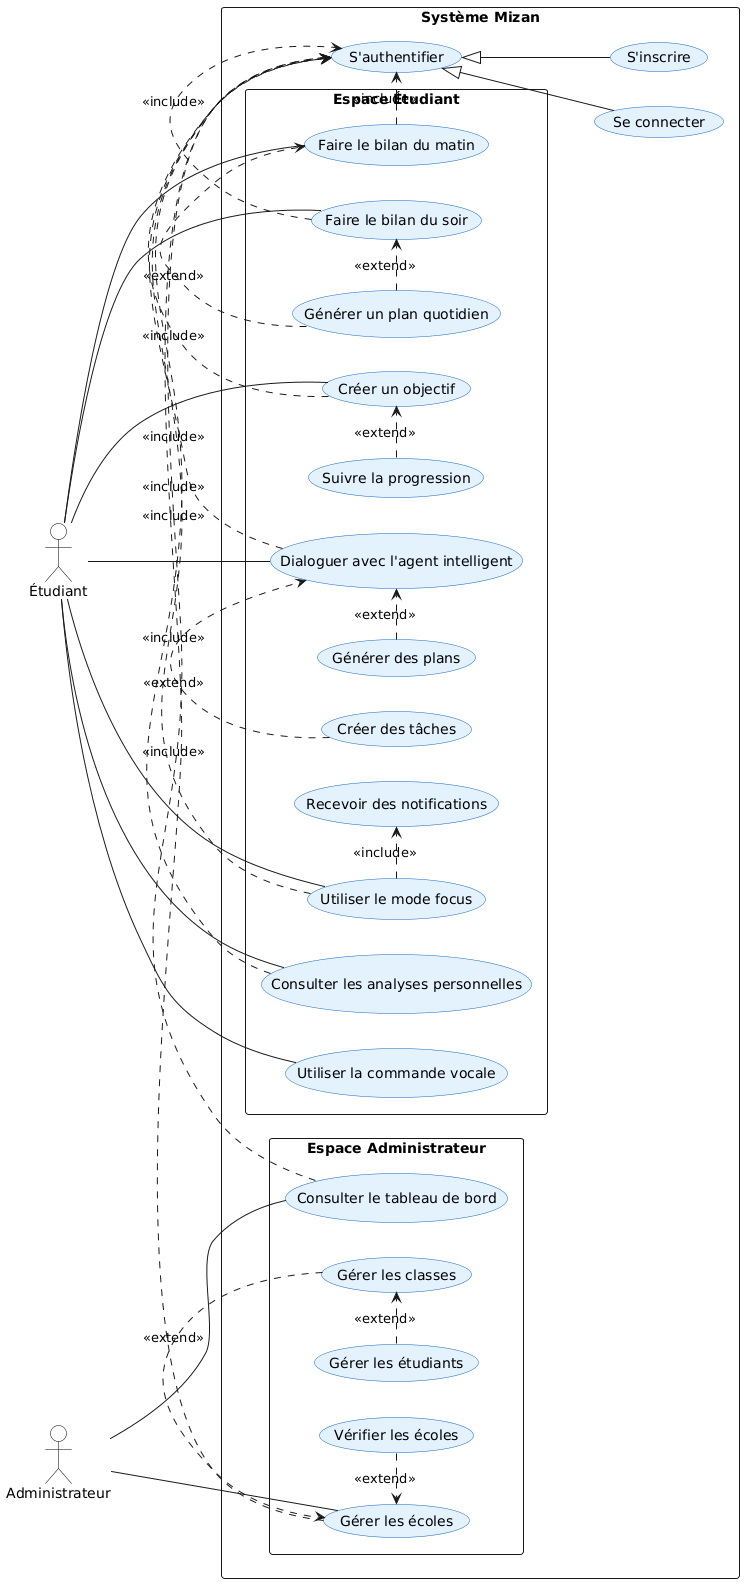
\includegraphics[width=0.92\textwidth,height=0.80\textheight,keepaspectratio]{figures/usecase_diagram_rapport.png}
}{%
\IfFileExists{figures/diagramme_cas_utilisation_mizan.png}{%
\includegraphics[width=0.98\textwidth]{figures/diagramme_cas_utilisation_mizan.png}
}{%
\resizebox{0.98\textwidth}{!}{
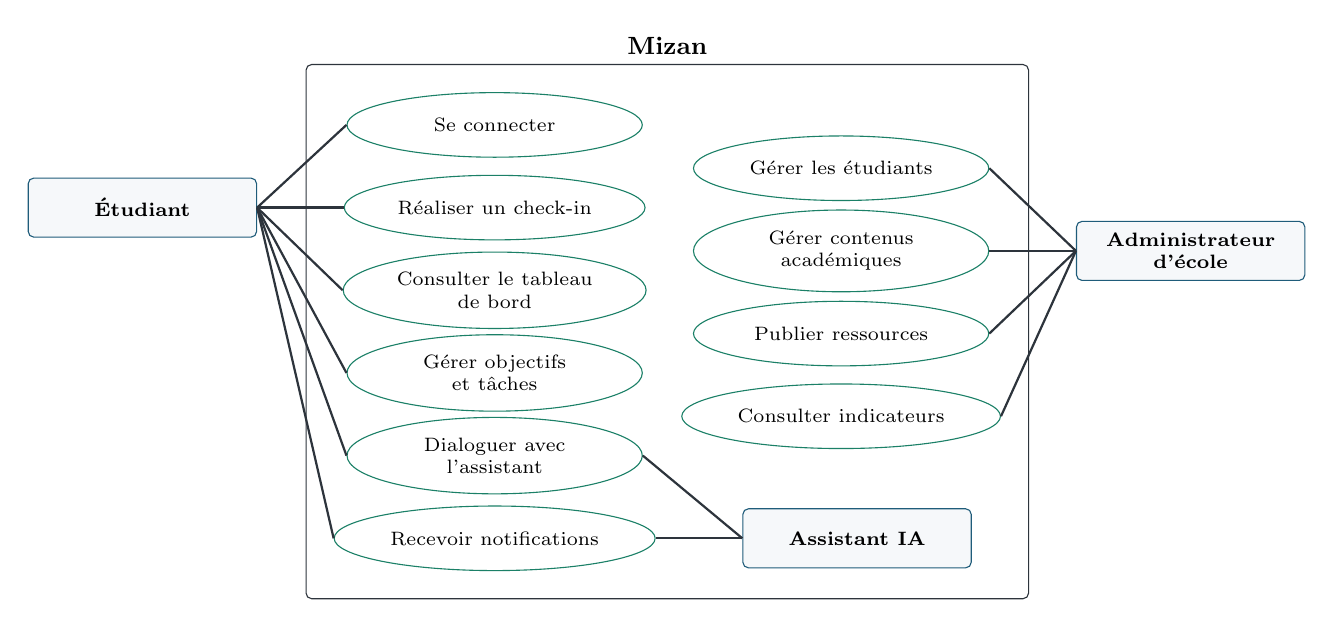
\begin{tikzpicture}[
    actor/.style={rectangle, rounded corners=2pt, draw=mizanblue, fill=softgray, minimum width=2.9cm, minimum height=0.75cm, align=center, font=\scriptsize\bfseries},
    usecase/.style={ellipse, draw=mizangreen, fill=white, minimum width=3.75cm, minimum height=0.82cm, align=center, font=\scriptsize},
    boundary/.style={rectangle, draw=darkgray, rounded corners=2pt, inner sep=0.35cm},
    assoc/.style={thick, color=darkgray}
]
\node[usecase] (login) at (3.6,2.3) {Se connecter};
\node[usecase] (checkin) at (3.6,1.25) {Réaliser un check-in};
\node[usecase] (dashboard) at (3.6,0.2) {Consulter le tableau\\de bord};
\node[usecase] (goals) at (3.6,-0.85) {Gérer objectifs\\et tâches};
\node[usecase] (chat) at (3.6,-1.9) {Dialoguer avec\\l'assistant};
\node[usecase] (notify) at (3.6,-2.95) {Recevoir notifications};
\node[usecase] (students) at (8.0,1.75) {Gérer les étudiants};
\node[usecase] (content) at (8.0,0.7) {Gérer contenus\\académiques};
\node[usecase] (resources) at (8.0,-0.35) {Publier ressources};
\node[usecase] (analytics) at (8.0,-1.4) {Consulter indicateurs};
\node[boundary, fit=(login)(checkin)(dashboard)(goals)(chat)(notify)(students)(content)(resources)(analytics), label={[font=\small\bfseries]above:Mizan}] (system) {};
\node[actor, left=1.1cm of checkin] (student) {Étudiant};
\node[actor, right=1.1cm of content] (admin) {Administrateur\\d'école};
\node[actor, right=1.1cm of notify] (ia) {Assistant IA};
\draw[assoc] (student.east) -- (login.west);
\draw[assoc] (student.east) -- (checkin.west);
\draw[assoc] (student.east) -- (dashboard.west);
\draw[assoc] (student.east) -- (goals.west);
\draw[assoc] (student.east) -- (chat.west);
\draw[assoc] (student.east) -- (notify.west);
\draw[assoc] (admin.west) -- (students.east);
\draw[assoc] (admin.west) -- (content.east);
\draw[assoc] (admin.west) -- (resources.east);
\draw[assoc] (admin.west) -- (analytics.east);
\draw[assoc] (ia.west) -- (chat.east);
\draw[assoc] (ia.west) -- (notify.east);
\end{tikzpicture}
}
}
}
\caption{Diagramme de cas d'utilisation de Mizan}
\end{figure}

La spécification suivante décrit les cas d'utilisation visibles dans le diagramme. Elle précise, pour chaque fonction importante, l'acteur concerné, la condition d'accès, le déroulement nominal et le résultat attendu. Cette description permet de transformer le diagramme en exigences fonctionnelles exploitables pendant la conception.

\begin{longtable}{@{}L{0.20\textwidth}L{0.18\textwidth}L{0.25\textwidth}L{0.27\textwidth}@{}}
\toprule
\textbf{Cas d'utilisation} & \textbf{Acteur} & \textbf{Précondition} & \textbf{Scénario nominal et postcondition} \\
\midrule
\endhead
S'inscrire & Étudiant & L'étudiant ne possède pas encore de compte actif. & Il renseigne ses informations, valide le formulaire et obtient un compte utilisable après contrôle des données. \\
Se connecter / s'authentifier & Étudiant, Administrateur & Le compte existe et les identifiants sont disponibles. & L'utilisateur saisit ses identifiants, le système vérifie l'accès et ouvre l'espace correspondant à son rôle. \\
Faire le bilan du matin & Étudiant & L'étudiant est authentifié. & Il saisit son humeur, son sommeil et ses priorités. Le système enregistre le bilan et prépare les données de suivi de la journée. \\
Faire le bilan du soir & Étudiant & L'étudiant est authentifié et peut avoir déjà réalisé un bilan du matin. & Il indique l'état de sa journée, les tâches réalisées et les difficultés rencontrées. Le système complète l'historique quotidien. \\
Générer un plan quotidien & Étudiant, Agent intelligent & Des informations de contexte sont disponibles. & Le système analyse les bilans, objectifs, tâches et échéances afin de proposer un plan adapté à la journée. \\
Créer un objectif & Étudiant & L'étudiant est connecté à son espace. & Il ajoute un objectif avec un titre, une description et éventuellement une priorité. L'objectif devient consultable et modifiable. \\
Suivre la progression & Étudiant & Des objectifs, tâches ou check-ins existent. & Le système affiche l'évolution des objectifs, l'état des tâches et les indicateurs personnels. \\
\bottomrule
\caption{Spécification des cas d'utilisation de l'espace étudiant}
\end{longtable}

\begin{longtable}{@{}L{0.20\textwidth}L{0.18\textwidth}L{0.25\textwidth}L{0.27\textwidth}@{}}
\toprule
\textbf{Cas d'utilisation} & \textbf{Acteur} & \textbf{Précondition} & \textbf{Scénario nominal et postcondition} \\
\midrule
\endhead
Dialoguer avec l'agent intelligent & Étudiant & L'étudiant est authentifié et dispose d'un contexte minimal. & Il pose une question. Le système prépare le contexte, interroge l'agent ou le fallback, puis retourne une réponse personnalisée. \\
Générer des plans & Étudiant, Agent intelligent & Les objectifs, tâches ou bilans peuvent être analysés. & L'agent propose des étapes concrètes pour organiser le travail, réduire la surcharge ou préparer une échéance. \\
Créer des tâches & Étudiant & L'étudiant est connecté. & Il crée une tâche liée à un objectif, un cours ou une priorité personnelle. La tâche est ajoutée au suivi. \\
Recevoir des notifications & Étudiant & Une action ou une condition de rappel est détectée. & Le système envoie un rappel ou une alerte liée aux objectifs, bilans, tâches ou recommandations. \\
Utiliser le mode focus & Étudiant & L'étudiant souhaite lancer une session de concentration. & Il démarre un mode de travail. Le système suit la session et peut l'associer à une tâche ou un objectif. \\
Consulter les analyses personnelles & Étudiant & Des données de suivi existent. & Le système présente des indicateurs sur l'humeur, le sommeil, la progression et les tendances personnelles. \\
\bottomrule
\caption{Spécification des cas d'utilisation d'accompagnement étudiant}
\end{longtable}

\begin{longtable}{@{}L{0.22\textwidth}L{0.18\textwidth}L{0.25\textwidth}L{0.25\textwidth}@{}}
\toprule
\textbf{Cas d'utilisation} & \textbf{Acteur} & \textbf{Précondition} & \textbf{Scénario nominal et postcondition} \\
\midrule
\endhead
Consulter le tableau de bord & Administrateur & L'administrateur est authentifié. & Il accède aux indicateurs de suivi et obtient une vue synthétique des données de l'établissement. \\
Gérer les classes & Administrateur & Une école ou une structure académique existe. & Il crée, modifie ou consulte les classes afin d'organiser les étudiants. \\
Gérer les étudiants & Administrateur & Les classes sont disponibles. & Il ajoute, importe, modifie ou consulte les profils étudiants rattachés à l'établissement. \\
Vérifier les écoles & Administrateur & Des écoles sont en attente de validation. & Il consulte les demandes, vérifie les informations et décide de l'acceptation ou du rejet. \\
Gérer les écoles & Administrateur & L'administrateur dispose des droits nécessaires. & Il administre les écoles, leurs informations et leur état de validation. \\
\bottomrule
\caption{Spécification des cas d'utilisation administrateur}
\end{longtable}

Dans ce diagramme, la relation \texttt{include} signifie qu'un cas d'utilisation dépend d'un comportement obligatoire. L'authentification est donc incluse dans la majorité des fonctionnalités protégées, car l'étudiant ou l'administrateur doit être identifié avant d'accéder aux données. La relation \texttt{extend} indique un comportement optionnel ou conditionnel : par exemple, le bilan du soir complète le suivi quotidien, la génération de plans enrichit l'utilisation de l'agent intelligent, et les notifications peuvent être déclenchées après certaines actions ou certains changements d'état.

\subsection{Cahier des charges}
\subsubsection*{Objectifs détaillés}
\addcontentsline{toc}{subsubsection}{Objectifs détaillés}
Le cahier des charges impose une plateforme multi-interfaces, sécurisée, modulaire, capable de gérer les étudiants, les contenus académiques, les check-ins, les objectifs, les ressources, l'assistant et les tableaux de bord.

\begin{itemize}
    \item garantir un accès sécurisé aux espaces étudiant et administrateur ;
    \item permettre la saisie rapide des check-ins depuis le web ou le mobile ;
    \item fournir une vision synthétique de la journée de l'étudiant ;
    \item offrir aux administrateurs des outils simples de gestion et d'import ;
    \item intégrer un assistant capable de fonctionner même en mode dégradé ;
    \item préparer un déploiement cloud reproductible.
\end{itemize}

\subsubsection*{Contraintes}
\addcontentsline{toc}{subsubsection}{Contraintes}
Les contraintes techniques incluent FastAPI, Next.js, React Native, PostgreSQL, Docker et CI/CD. Les contraintes logicielles portent sur la validation des données et la sécurité. Les contraintes temporelles imposent une progression par modules prioritaires.

\subsubsection*{Critères d'acceptation}
\addcontentsline{toc}{subsubsection}{Critères d'acceptation}
Une première version de Mizan est considérée comme acceptable si l'étudiant peut se connecter, réaliser un check-in, consulter son tableau de bord et suivre au moins un objectif. L'administrateur doit pouvoir gérer une structure institutionnelle, ajouter des étudiants et créer des contenus académiques. Le système doit refuser les accès non autorisés, valider les données reçues, conserver les historiques et rester utilisable lorsque le fournisseur IA n'est pas configuré.

Les critères d'acceptation incluent aussi la lisibilité de l'interface, la cohérence des messages d'erreur, la possibilité d'exécuter les tests automatiquement et la capacité à produire un build front-end sans erreur. Le scénario minimal attendu est : création d'un étudiant, connexion, check-in, consultation du tableau de bord, interaction avec l'assistant et consultation d'un indicateur administrateur.

% ===========================================================
% CHAPITRE 3
% ===========================================================

\section{Conception de la Solution}
\subsection{Architecture générale}
\subsubsection{Diagramme de contexte système C4 -- Niveau 1}
\begin{figure}[H]
\centering
\IfFileExists{figures/diagramme_c4_contexte_mizan.png}{%
\includegraphics[width=0.95\textwidth]{figures/diagramme_c4_contexte_mizan.png}
}{%
\resizebox{0.95\textwidth}{!}{
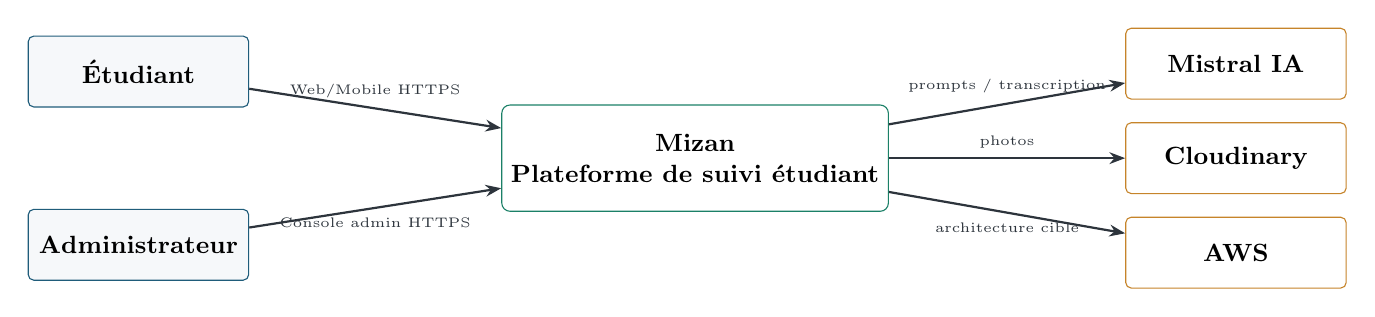
\begin{tikzpicture}[
    person/.style={rectangle, rounded corners=2pt, draw=mizanblue, fill=softgray, minimum width=2.8cm, minimum height=0.9cm, align=center, font=\small\bfseries},
    system/.style={rectangle, rounded corners=3pt, draw=mizangreen, fill=white, minimum width=4.2cm, minimum height=1.35cm, align=center, font=\small\bfseries},
    ext/.style={rectangle, rounded corners=2pt, draw=mizanamber, fill=white, minimum width=2.8cm, minimum height=0.9cm, align=center, font=\small\bfseries},
    arrow/.style={-{Stealth[length=2mm]}, thick, color=darkgray}
]
\node[system] (mizan) {Mizan\\Plateforme de suivi étudiant};
\node[person, left=3.2cm of mizan, yshift=1.1cm] (student) {Étudiant};
\node[person, left=3.2cm of mizan, yshift=-1.1cm] (admin) {Administrateur};
\node[ext, right=3.0cm of mizan, yshift=1.2cm] (mistral) {Mistral IA};
\node[ext, right=3.0cm of mizan] (cloudinary) {Cloudinary};
\node[ext, right=3.0cm of mizan, yshift=-1.2cm] (aws) {AWS};
\draw[arrow] (student) -- node[above, font=\tiny]{Web/Mobile HTTPS} (mizan);
\draw[arrow] (admin) -- node[below, font=\tiny]{Console admin HTTPS} (mizan);
\draw[arrow] (mizan) -- node[above, font=\tiny]{prompts / transcription} (mistral);
\draw[arrow] (mizan) -- node[above, font=\tiny]{photos} (cloudinary);
\draw[arrow] (mizan) -- node[below, font=\tiny]{architecture cible} (aws);
\end{tikzpicture}
}
}
\caption{Diagramme de contexte système C4 niveau 1}
\end{figure}

\subsubsection{Diagramme de conteneurs C4 -- Niveau 2}
\begin{figure}[H]
\centering
\IfFileExists{figures/diagramme_c4_conteneurs_mizan.png}{%
\includegraphics[width=0.98\textwidth]{figures/diagramme_c4_conteneurs_mizan.png}
}{%
\resizebox{0.98\textwidth}{!}{
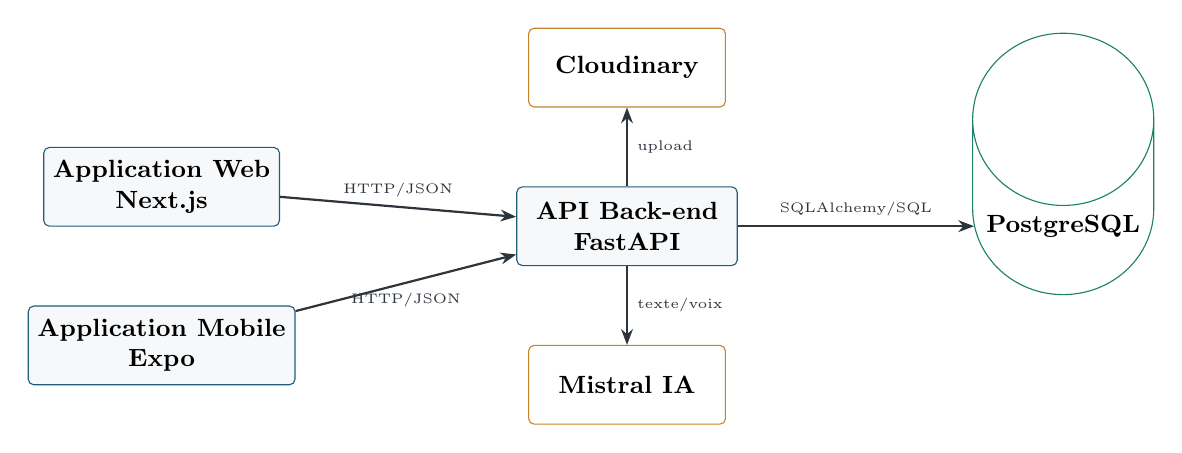
\begin{tikzpicture}[
    container/.style={rectangle, rounded corners=2pt, draw=mizanblue, fill=softgray, minimum width=2.8cm, minimum height=1cm, align=center, font=\small\bfseries},
    store/.style={cylinder, shape border rotate=90, draw=mizangreen, fill=white, minimum width=2.3cm, minimum height=1.2cm, align=center, font=\small\bfseries},
    ext/.style={rectangle, rounded corners=2pt, draw=mizanamber, fill=white, minimum width=2.5cm, minimum height=1cm, align=center, font=\small\bfseries},
    arrow/.style={-{Stealth[length=2mm]}, thick, color=darkgray}
]
\node[container] (web) {Application Web\\Next.js};
\node[container, below=1.0cm of web] (mobile) {Application Mobile\\Expo};
\node[container, right=3.0cm of web, yshift=-0.5cm] (api) {API Back-end\\FastAPI};
\node[store, right=3.0cm of api] (db) {PostgreSQL};
\node[ext, above=1.0cm of api] (cloudinary) {Cloudinary};
\node[ext, below=1.0cm of api] (mistral) {Mistral IA};
\draw[arrow] (web) -- node[above, font=\tiny]{HTTP/JSON} (api);
\draw[arrow] (mobile) -- node[below, font=\tiny]{HTTP/JSON} (api);
\draw[arrow] (api) -- node[above, font=\tiny]{SQLAlchemy/SQL} (db);
\draw[arrow] (api) -- node[right, font=\tiny]{upload} (cloudinary);
\draw[arrow] (api) -- node[right, font=\tiny]{texte/voix} (mistral);
\end{tikzpicture}
}
}
\caption{Diagramme de conteneurs C4 niveau 2}
\end{figure}

\subsubsection{Architecture matérielle cible}
L'architecture matérielle cible repose sur AWS. Le front-end et le back-end sont prévus sous forme de conteneurs ECS Fargate. La base PostgreSQL est prévue dans RDS. CloudFront et l'Application Load Balancer constituent les points d'entrée prévus pour l'exposition publique.

\subsubsection{Architecture réseau cible}
Le trafic utilisateur est prévu en HTTPS vers CloudFront puis vers l'Application Load Balancer. Les routes API sont redirigées vers le service back-end, tandis que les autres routes servent l'application front-end. La base RDS reste privée et accessible uniquement par le back-end.

\subsection{Choix technologiques}
\begin{longtable}{@{}L{0.24\textwidth}L{0.26\textwidth}L{0.40\textwidth}@{}}
\toprule
\textbf{Domaine} & \textbf{Choix} & \textbf{Justification} \\
\midrule
\endhead
Langage back-end & Python & Écosystème riche, lisibilité et intégration rapide avec FastAPI. \\
Framework API & FastAPI & Performance, validation Pydantic et documentation automatique. \\
Front-end web & Next.js / React & Architecture moderne, routage clair et TypeScript. \\
Mobile & Expo React Native & Développement mobile rapide et multi-plateforme. \\
SGBD & PostgreSQL & Robustesse, relations fortes et compatibilité SQLAlchemy. \\
Déploiement & Docker, Terraform, AWS & Reproductibilité, infrastructure versionnée et cloud managé. \\
\bottomrule
\caption{Choix technologiques et justification}
\end{longtable}

\subsection{Conception fonctionnelle}
\subsubsection{Diagramme de composants C4 -- Niveau 3}
\begin{figure}[H]
\centering
\IfFileExists{figures/diagramme_c4_composants_backend.png}{%
\includegraphics[width=0.98\textwidth]{figures/diagramme_c4_composants_backend.png}
}{%
\resizebox{0.98\textwidth}{!}{
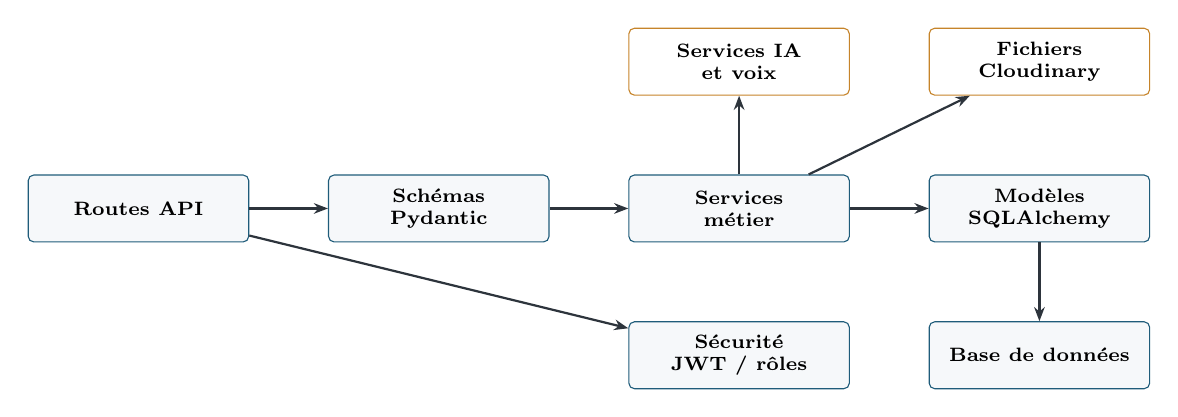
\begin{tikzpicture}[
    comp/.style={rectangle, rounded corners=2pt, draw=mizanblue, fill=softgray, minimum width=2.8cm, minimum height=0.85cm, align=center, font=\scriptsize\bfseries},
    ext/.style={rectangle, rounded corners=2pt, draw=mizanamber, fill=white, minimum width=2.8cm, minimum height=0.85cm, align=center, font=\scriptsize\bfseries},
    arrow/.style={-{Stealth[length=1.8mm]}, thick, color=darkgray}
]
\node[comp] (routes) {Routes API};
\node[comp, right=1.0cm of routes] (schemas) {Schémas\\Pydantic};
\node[comp, right=1.0cm of schemas] (services) {Services\\métier};
\node[comp, right=1.0cm of services] (models) {Modèles\\SQLAlchemy};
\node[comp, below=1.0cm of services] (security) {Sécurité\\JWT / rôles};
\node[comp, below=1.0cm of models] (db) {Base de données};
\node[ext, above=1.0cm of services] (agent) {Services IA\\et voix};
\node[ext, above=1.0cm of models] (files) {Fichiers\\Cloudinary};
\draw[arrow] (routes) -- (schemas);
\draw[arrow] (schemas) -- (services);
\draw[arrow] (services) -- (models);
\draw[arrow] (models) -- (db);
\draw[arrow] (routes) -- (security);
\draw[arrow] (services) -- (agent);
\draw[arrow] (services) -- (files);
\end{tikzpicture}
}
}
\caption{Diagramme de composants du back-end C4 niveau 3}
\end{figure}

\subsubsection{Répartition et rôle de chaque module}
Le dossier \texttt{routes/} expose les points d'accès HTTP. Le dossier \texttt{schemas/} valide les entrées et sorties. Le dossier \texttt{models/} représente les tables SQLAlchemy. Le dossier \texttt{services/} contient les règles métier. Le dossier \texttt{core/} centralise la configuration, la sécurité et la connexion à la base.

\subsubsection{Flux de circulation des données}
Les données saisies par l'utilisateur passent du front-end vers l'API. L'API valide la requête, applique les règles métier, persiste les données dans PostgreSQL et retourne une réponse structurée. Pour les fonctionnalités intelligentes, l'API construit un contexte et interroge le fournisseur IA.

Le flux de données est organisé de manière à conserver une séparation claire entre l'affichage, la validation, la logique métier et la persistance. Cette organisation limite les effets de bord : une modification de l'interface ne doit pas modifier directement les règles métier, et une évolution de la base de données doit passer par les modèles et les migrations. Les échanges entre les applications clientes et l'API utilisent principalement JSON sur HTTP, ce qui facilite l'intégration web et mobile.

\begin{longtable}{@{}L{0.24\textwidth}L{0.34\textwidth}L{0.32\textwidth}@{}}
\toprule
\textbf{Flux} & \textbf{Étapes principales} & \textbf{Résultat attendu} \\
\midrule
\endhead
Check-in étudiant & Saisie mobile ou web, validation Pydantic, sauvegarde PostgreSQL, mise à jour de l'historique. & État quotidien enregistré et exploitable par le tableau de bord. \\
Assistant intelligent & Construction du contexte, sélection des données utiles, appel IA ou fallback local, retour structuré. & Conseil contextualisé, plan d'action ou résumé de journée. \\
Import CSV & Téléversement, validation du fichier, lecture des lignes, création contrôlée des étudiants. & Réduction de la saisie manuelle et cohérence des comptes. \\
Notification & Déclenchement par action utilisateur ou agent, création en base, consultation REST ou temps réel. & Rappel visible par l'étudiant sans interrompre le parcours principal. \\
Tableau de bord & Agrégation des check-ins, objectifs, tâches, échéances et modes. & Vue synthétique de la situation académique et personnelle. \\
\bottomrule
\caption{Flux fonctionnels détaillés}
\end{longtable}

Pour éviter la duplication de logique, les traitements communs sont centralisés dans les services. Par exemple, la préparation du contexte étudiant est utilisée par l'assistant, les notifications et certains indicateurs du tableau de bord. Ainsi, l'application garde une source de vérité cohérente pour les informations sensibles comme les échéances, les objectifs et les derniers check-ins.

\subsection{Conception technique}
\subsubsection{Diagramme de code C4 -- Niveau 4}
\begin{figure}[H]
\centering
\IfFileExists{figures/diagramme_c4_code_checkin.png}{%
\includegraphics[width=0.96\textwidth]{figures/diagramme_c4_code_checkin.png}
}{%
\resizebox{0.96\textwidth}{!}{
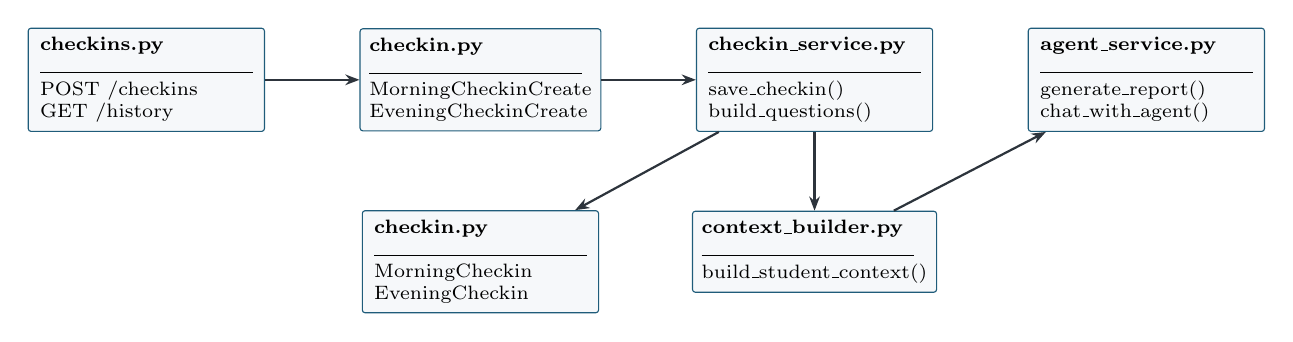
\begin{tikzpicture}[
    code/.style={rectangle, rounded corners=1pt, draw=mizanblue, fill=softgray, minimum width=3.0cm, align=left, font=\scriptsize},
    arrow/.style={-{Stealth[length=1.8mm]}, thick, color=darkgray}
]
\node[code] (route) {\textbf{checkins.py}\\\rule{2.7cm}{0.25pt}\\POST /checkins\\GET /history};
\node[code, right=1.2cm of route] (schema) {\textbf{checkin.py}\\\rule{2.7cm}{0.25pt}\\MorningCheckinCreate\\EveningCheckinCreate};
\node[code, right=1.2cm of schema] (service) {\textbf{checkin\_service.py}\\\rule{2.7cm}{0.25pt}\\save\_checkin()\\build\_questions()};
\node[code, below=1.0cm of service] (context) {\textbf{context\_builder.py}\\\rule{2.7cm}{0.25pt}\\build\_student\_context()};
\node[code, right=1.2cm of service] (agent) {\textbf{agent\_service.py}\\\rule{2.7cm}{0.25pt}\\generate\_report()\\chat\_with\_agent()};
\node[code, below=1.0cm of schema] (model) {\textbf{checkin.py}\\\rule{2.7cm}{0.25pt}\\MorningCheckin\\EveningCheckin};
\draw[arrow] (route) -- (schema);
\draw[arrow] (schema) -- (service);
\draw[arrow] (service) -- (model);
\draw[arrow] (service) -- (context);
\draw[arrow] (context) -- (agent);
\end{tikzpicture}
}
}
\caption{Diagramme de code C4 niveau 4 du module check-in}
\end{figure}

\subsubsection{Structure des dossiers}
\begin{lstlisting}
mizan/
|-- mizan-backend/        # API FastAPI, models, schemas, services, tests
|-- mizan-frontend/       # Application web Next.js
|-- mizan-mobile-app/     # Application mobile Expo React Native
|-- infra/aws/            # Infrastructure Terraform AWS
|-- docker/               # Configuration Docker et nginx
|-- .github/workflows/    # CI/CD GitHub Actions
|-- rapport/              # Rapport LaTeX
\end{lstlisting}

\subsubsection{Organisation des classes et interaction entre modules}
Les classes ORM représentent les entités persistantes. Les schémas Pydantic assurent la validation. Les services orchestrent les interactions entre modèles, contexte et fournisseurs externes. Ce découpage reprend les principes MVC et service layer.

\begin{longtable}{@{}L{0.25\textwidth}L{0.35\textwidth}L{0.30\textwidth}@{}}
\toprule
\textbf{Principe} & \textbf{Application dans Mizan} & \textbf{Apport} \\
\midrule
\endhead
Repository implicite & Les requêtes SQLAlchemy sont regroupées dans les services ou fonctions spécialisées. & Limite la dispersion des accès à la base. \\
Service layer & Les règles métier sont placées dans \texttt{services/}. & Facilite les tests et l'évolution des modules. \\
DTO / Schémas & Les entrées et sorties passent par Pydantic. & Réduit les erreurs de format et documente les contrats API. \\
Middleware de sécurité & Les dépendances FastAPI identifient l'utilisateur et son rôle. & Protège les routes sans répéter le même code. \\
Fallback applicatif & L'assistant peut répondre en mode local si le fournisseur IA est absent. & Améliore la disponibilité fonctionnelle. \\
\bottomrule
\caption{Principes de conception appliqués}
\end{longtable}

L'interaction entre modules suit généralement le même enchaînement : une route reçoit la demande, un schéma valide les données, un service applique les règles, un modèle interagit avec PostgreSQL, puis une réponse normalisée est renvoyée. Ce chemin rend le comportement plus prévisible, surtout pour les fonctionnalités qui combinent plusieurs sources de données.

\subsection{Modélisation UML}
La modélisation UML décrit la structure interne du domaine métier et complète les vues C4. Les diagrammes C4 expliquent l'architecture par niveaux, tandis que l'UML précise les entités, leurs relations et certains échanges dynamiques. Dans Mizan, cette modélisation est utile pour relier les fonctionnalités aux données persistées : utilisateur, étudiant, classe, check-ins, objectifs, tâches, ressources, notifications et décisions de l'assistant.

\begin{longtable}{@{}L{0.27\textwidth}L{0.34\textwidth}L{0.29\textwidth}@{}}
\toprule
\textbf{Diagramme UML} & \textbf{Rôle dans le rapport} & \textbf{Information apportée} \\
\midrule
\endhead
Cas d'utilisation & Synthétiser les interactions entre acteurs et système. & Fonctions accessibles à l'étudiant, à l'administrateur et à l'assistant IA. \\
Classes & Structurer le domaine persistant. & Entités principales, attributs importants et cardinalités. \\
Séquence & Montrer les échanges pendant un scénario. & Ordre des appels entre front-end, API, base, contexte et assistant. \\
\bottomrule
\caption{Rôle des diagrammes UML dans Mizan}
\end{longtable}

\subsubsection{Diagrammes de séquence}
Les diagrammes de séquence complètent le diagramme de classes en décrivant l'ordre des échanges entre les acteurs, les interfaces, l'API, les services métier et la base de données. Ils permettent de vérifier que la conception technique reste cohérente avec les cas d'utilisation : chaque action utilisateur passe par une interface, une validation côté API, un traitement métier, puis une réponse exploitable.

Le scénario retenu est le check-in étudiant avec analyse intelligente, car il représente le coeur de l'expérience Mizan : l'étudiant saisit son état quotidien, le système enregistre les données, construit un contexte récent, puis prépare une réponse d'accompagnement exploitable. Ce flux montre à la fois l'interaction utilisateur, la validation côté API, la persistance des données et l'appel au service intelligent.

\begin{figure}[H]
\centering
\IfFileExists{figures/checkin_seq_uml.png}{%
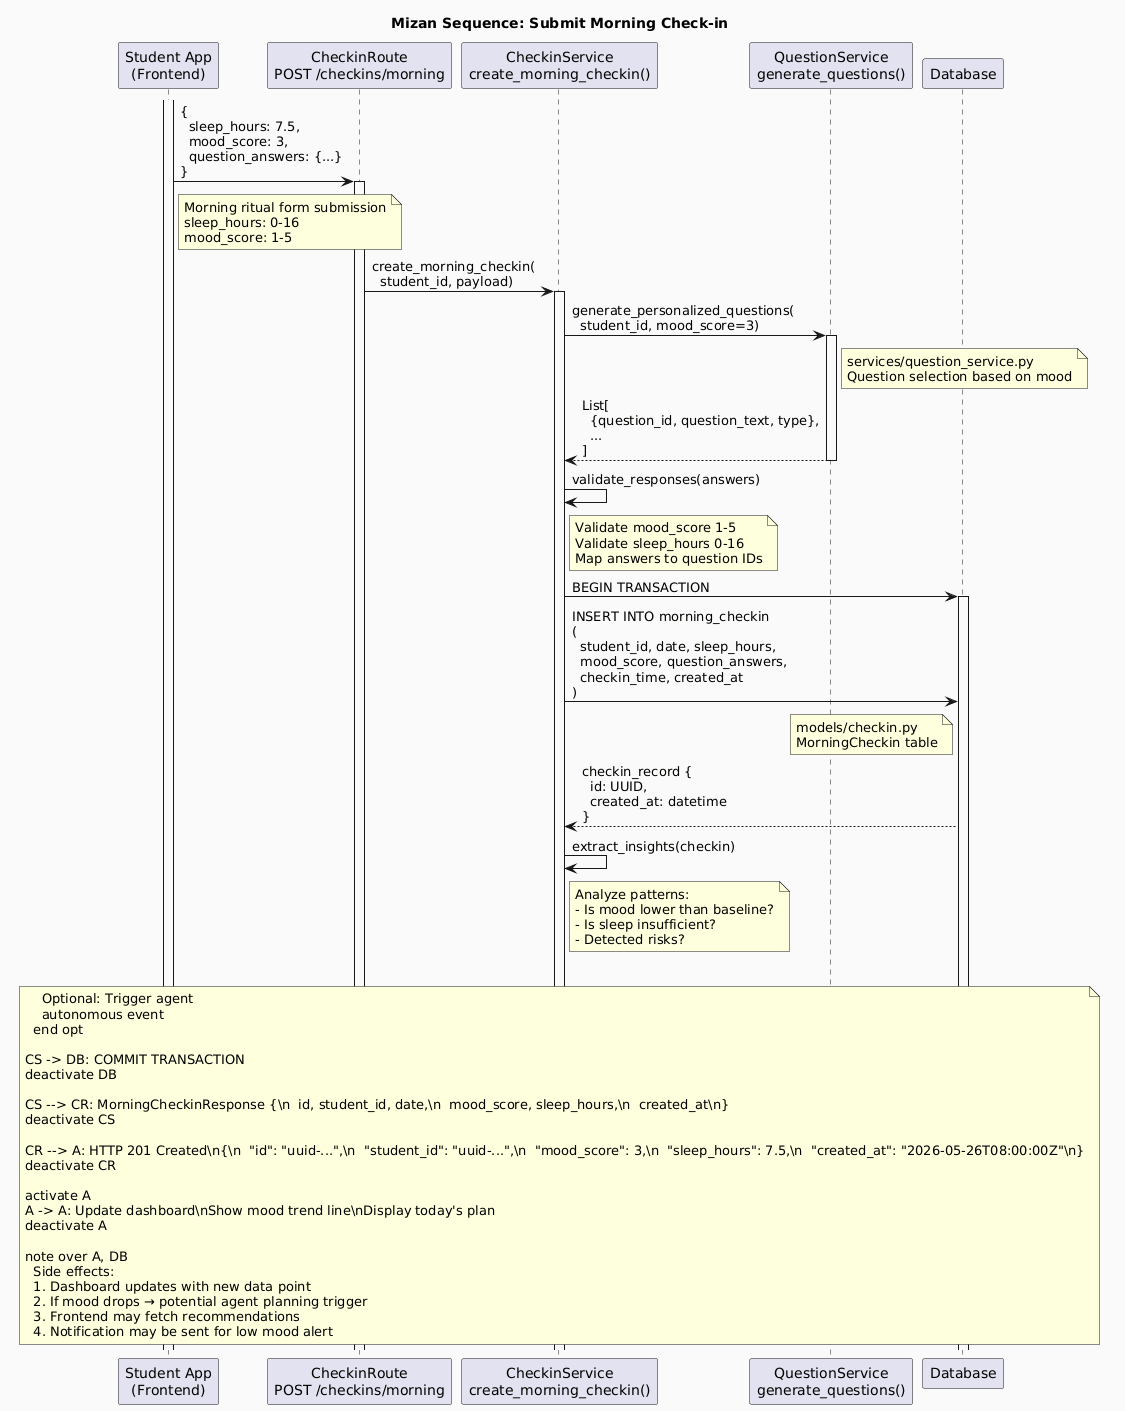
\includegraphics[width=0.96\textwidth,height=0.78\textheight,keepaspectratio]{figures/checkin_seq_uml.png}
}{%
\IfFileExists{figures/diagramme_sequence_checkin_ia.png}{%
\includegraphics[width=0.98\textwidth]{figures/diagramme_sequence_checkin_ia.png}
}{%
\resizebox{0.98\textwidth}{!}{
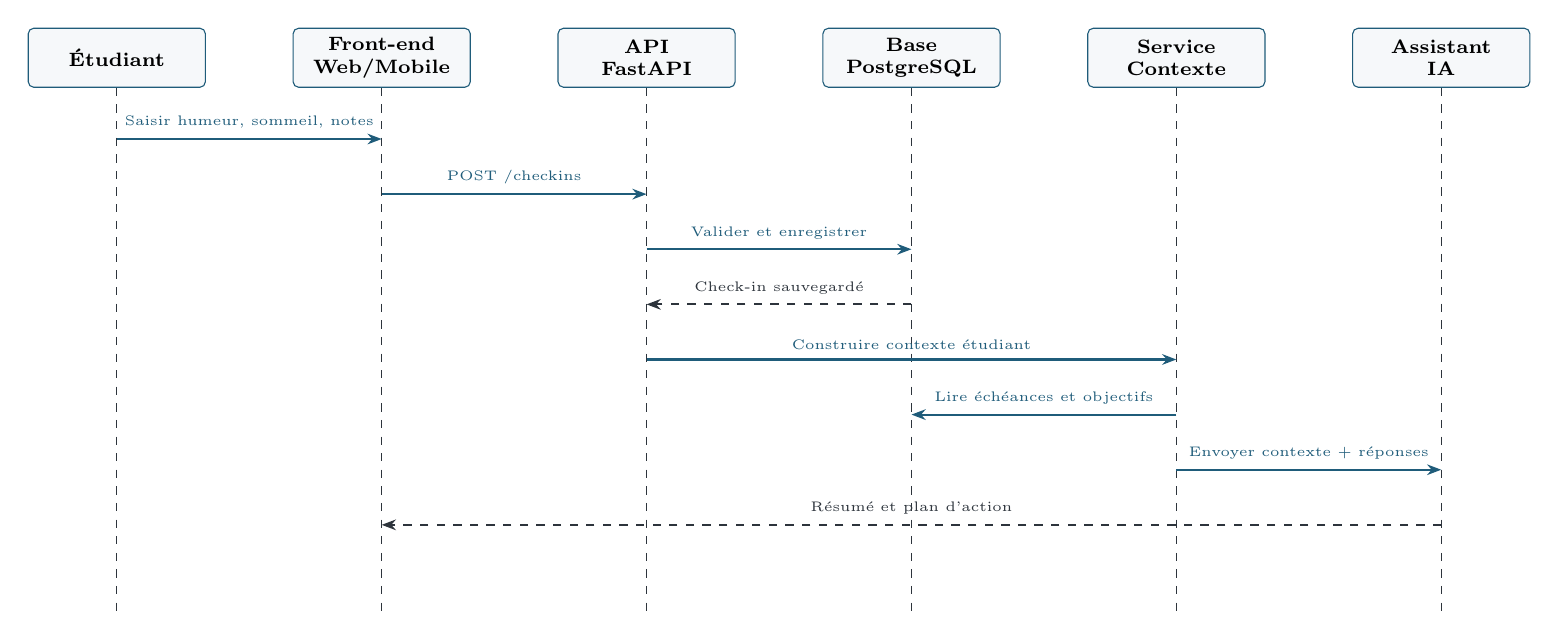
\begin{tikzpicture}[
    participant/.style={rectangle, draw=mizanblue, fill=softgray, rounded corners=2pt, minimum width=2.25cm, minimum height=0.75cm, align=center, font=\scriptsize\bfseries},
    call/.style={-{Stealth[length=1.8mm]}, thick, color=mizanblue},
    return/.style={-{Stealth[length=1.8mm]}, dashed, thick, color=darkgray},
    life/.style={dashed, color=darkgray}
]
\node[participant] (student) {Étudiant};
\node[participant, right=1.1cm of student] (front) {Front-end\\Web/Mobile};
\node[participant, right=1.1cm of front] (api) {API\\FastAPI};
\node[participant, right=1.1cm of api] (db) {Base\\PostgreSQL};
\node[participant, right=1.1cm of db] (context) {Service\\Contexte};
\node[participant, right=1.1cm of context] (agent) {Assistant\\IA};
\foreach \p in {student,front,api,db,context,agent} {
    \draw[life] (\p.south) -- ++(0,-6.7cm);
}
\coordinate (y1) at ($(student.south)+(0,-0.65cm)$);
\coordinate (y2) at ($(student.south)+(0,-1.35cm)$);
\coordinate (y3) at ($(student.south)+(0,-2.05cm)$);
\coordinate (y4) at ($(student.south)+(0,-2.75cm)$);
\coordinate (y5) at ($(student.south)+(0,-3.45cm)$);
\coordinate (y6) at ($(student.south)+(0,-4.15cm)$);
\coordinate (y7) at ($(student.south)+(0,-4.85cm)$);
\coordinate (y8) at ($(student.south)+(0,-5.55cm)$);
\draw[call] (student |- y1) -- node[above, font=\tiny]{Saisir humeur, sommeil, notes} (front |- y1);
\draw[call] (front |- y2) -- node[above, font=\tiny]{POST /checkins} (api |- y2);
\draw[call] (api |- y3) -- node[above, font=\tiny]{Valider et enregistrer} (db |- y3);
\draw[return] (db |- y4) -- node[above, font=\tiny]{Check-in sauvegardé} (api |- y4);
\draw[call] (api |- y5) -- node[above, font=\tiny]{Construire contexte étudiant} (context |- y5);
\draw[call] (context |- y6) -- node[above, font=\tiny]{Lire échéances et objectifs} (db |- y6);
\draw[call] (context |- y7) -- node[above, font=\tiny]{Envoyer contexte + réponses} (agent |- y7);
\draw[return] (agent |- y8) -- node[above, font=\tiny]{Résumé et plan d'action} (front |- y8);
\end{tikzpicture}
}
}
}
\caption{Diagramme de séquence du check-in avec analyse intelligente}
\end{figure}

Ce diagramme montre que le check-in n'est pas seulement un formulaire enregistré en base. Après la validation, les données saisies servent à construire un contexte étudiant. Ce contexte regroupe les informations récentes utiles, puis il est transmis à l'assistant afin de produire un résumé, un conseil ou un plan d'action. Si le fournisseur IA n'est pas disponible, le service peut appliquer un mode de secours local afin de conserver une réponse minimale pour l'utilisateur.

\subsubsection{Diagramme de classes}
Le diagramme de classes représente une vue simplifiée du modèle de données. Il montre que l'entité \texttt{User} porte l'identité et le rôle, tandis que \texttt{Student} décrit le profil académique rattaché à une classe. Les entités comme \texttt{Checkin}, \texttt{Goal}, \texttt{Task} et \texttt{ModeSession} appartiennent à l'étudiant et alimentent le suivi quotidien. Les entités \texttt{AgentRun}, \texttt{Notification} et \texttt{Resource} servent à transformer ce suivi en accompagnement exploitable.

\begin{figure}[H]
\centering
\IfFileExists{figures/class_diagram_rapport.png}{%
\makebox[\textwidth][c]{\rotatebox{90}{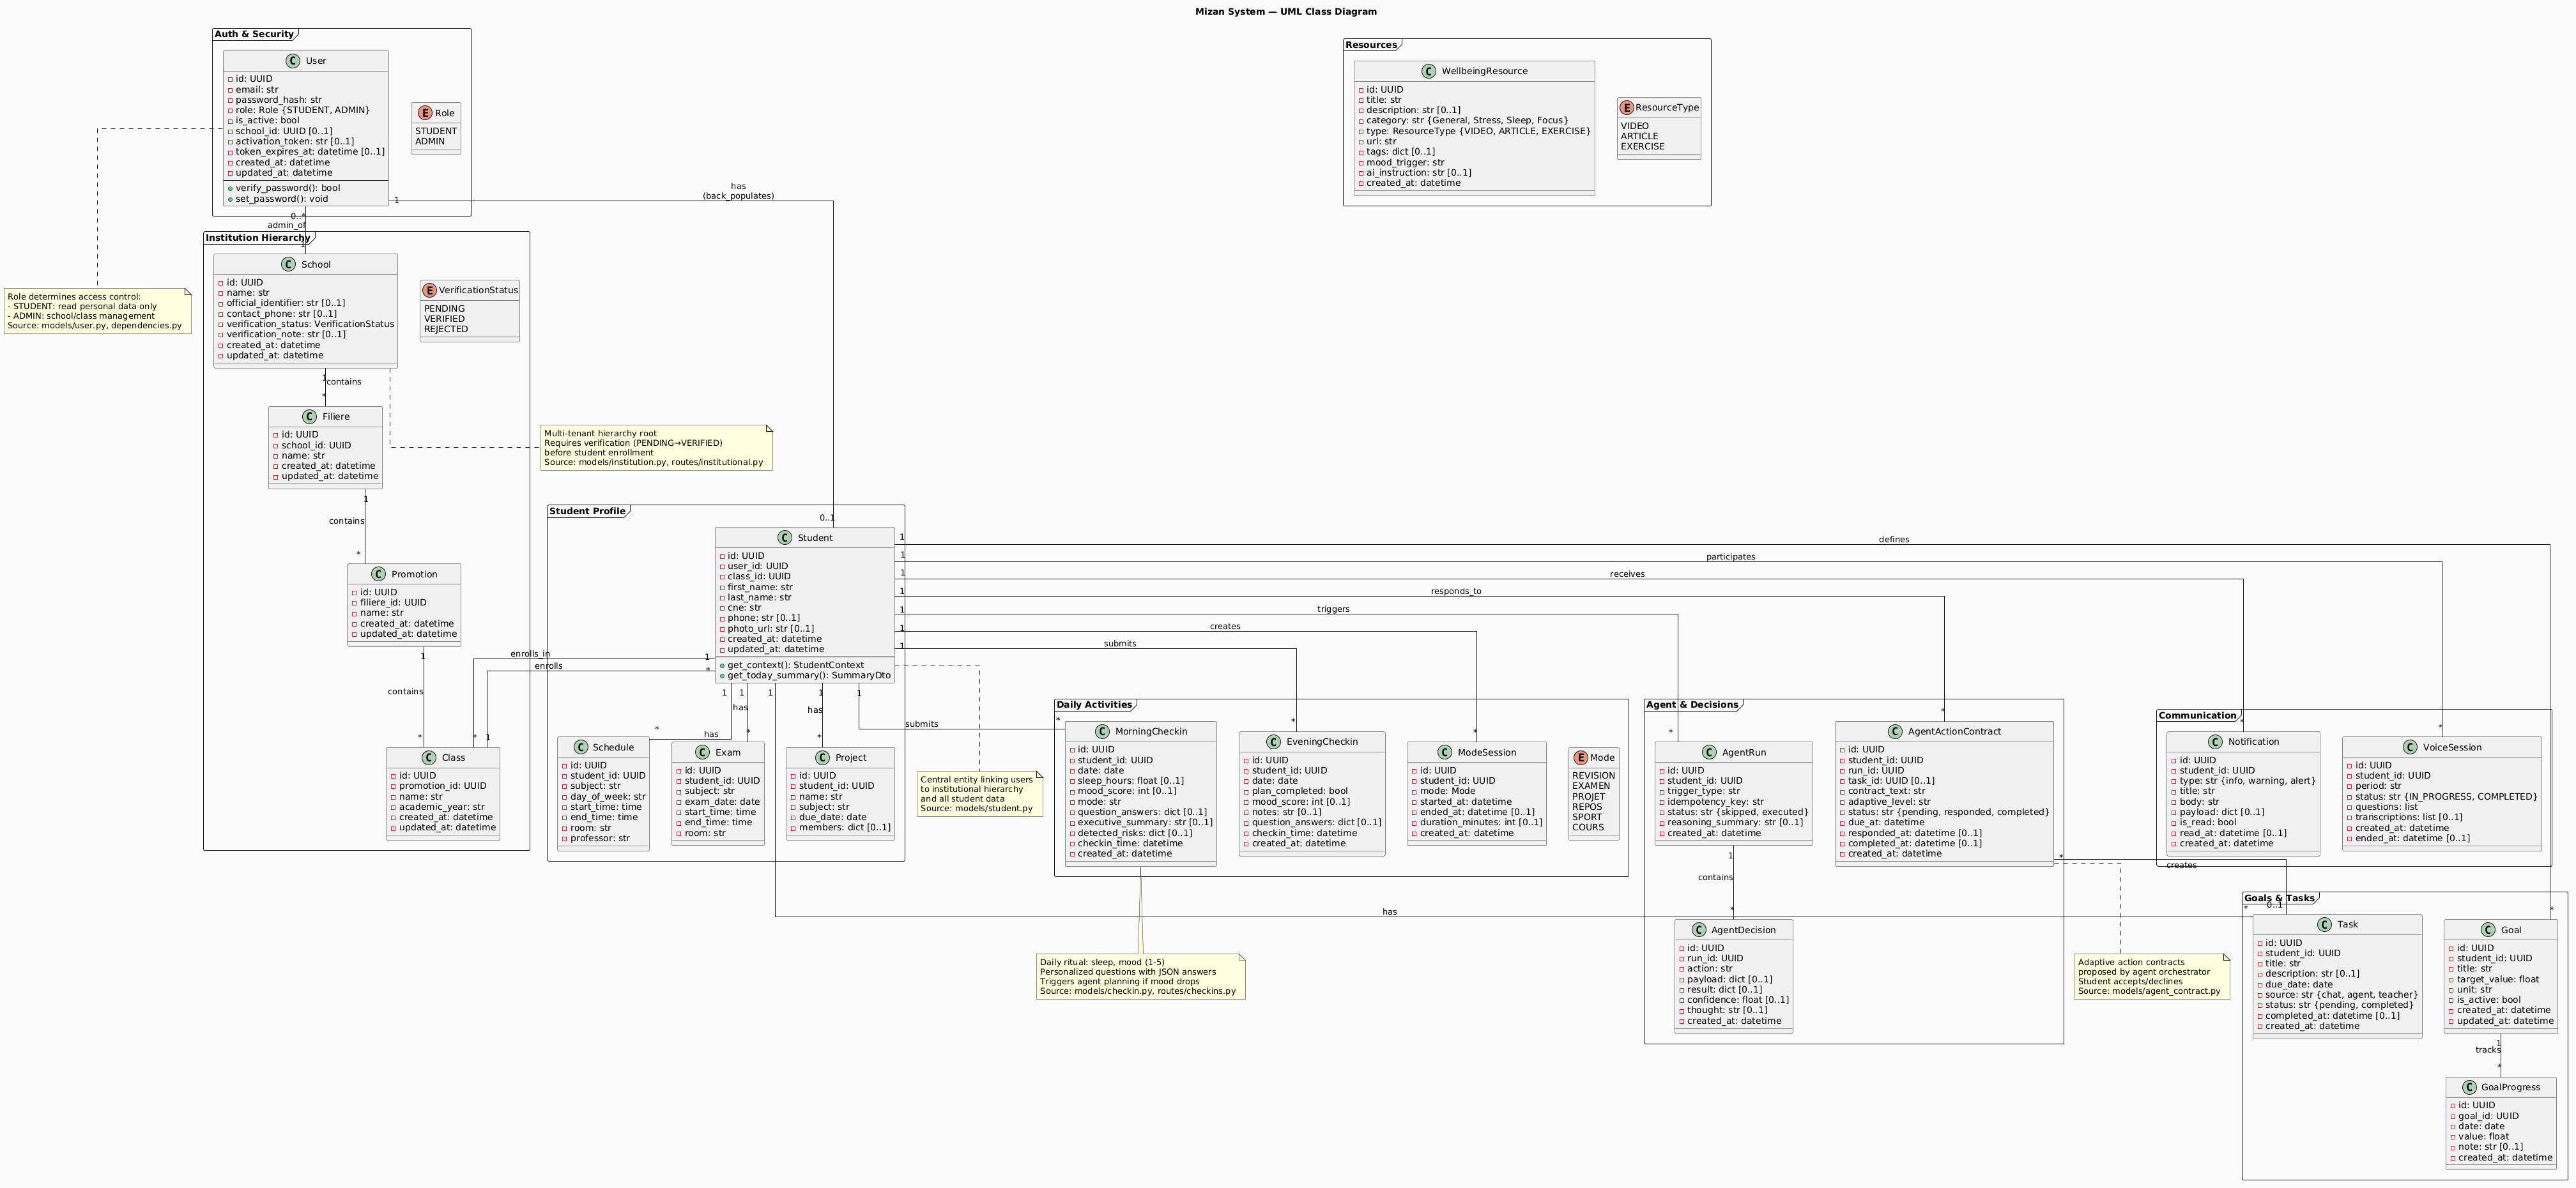
\includegraphics[width=0.92\textheight,height=0.92\textwidth,keepaspectratio]{figures/class_diagram_rapport.png}}}
}{%
\IfFileExists{figures/uml-class.png}{%
\makebox[\textwidth][c]{\rotatebox{90}{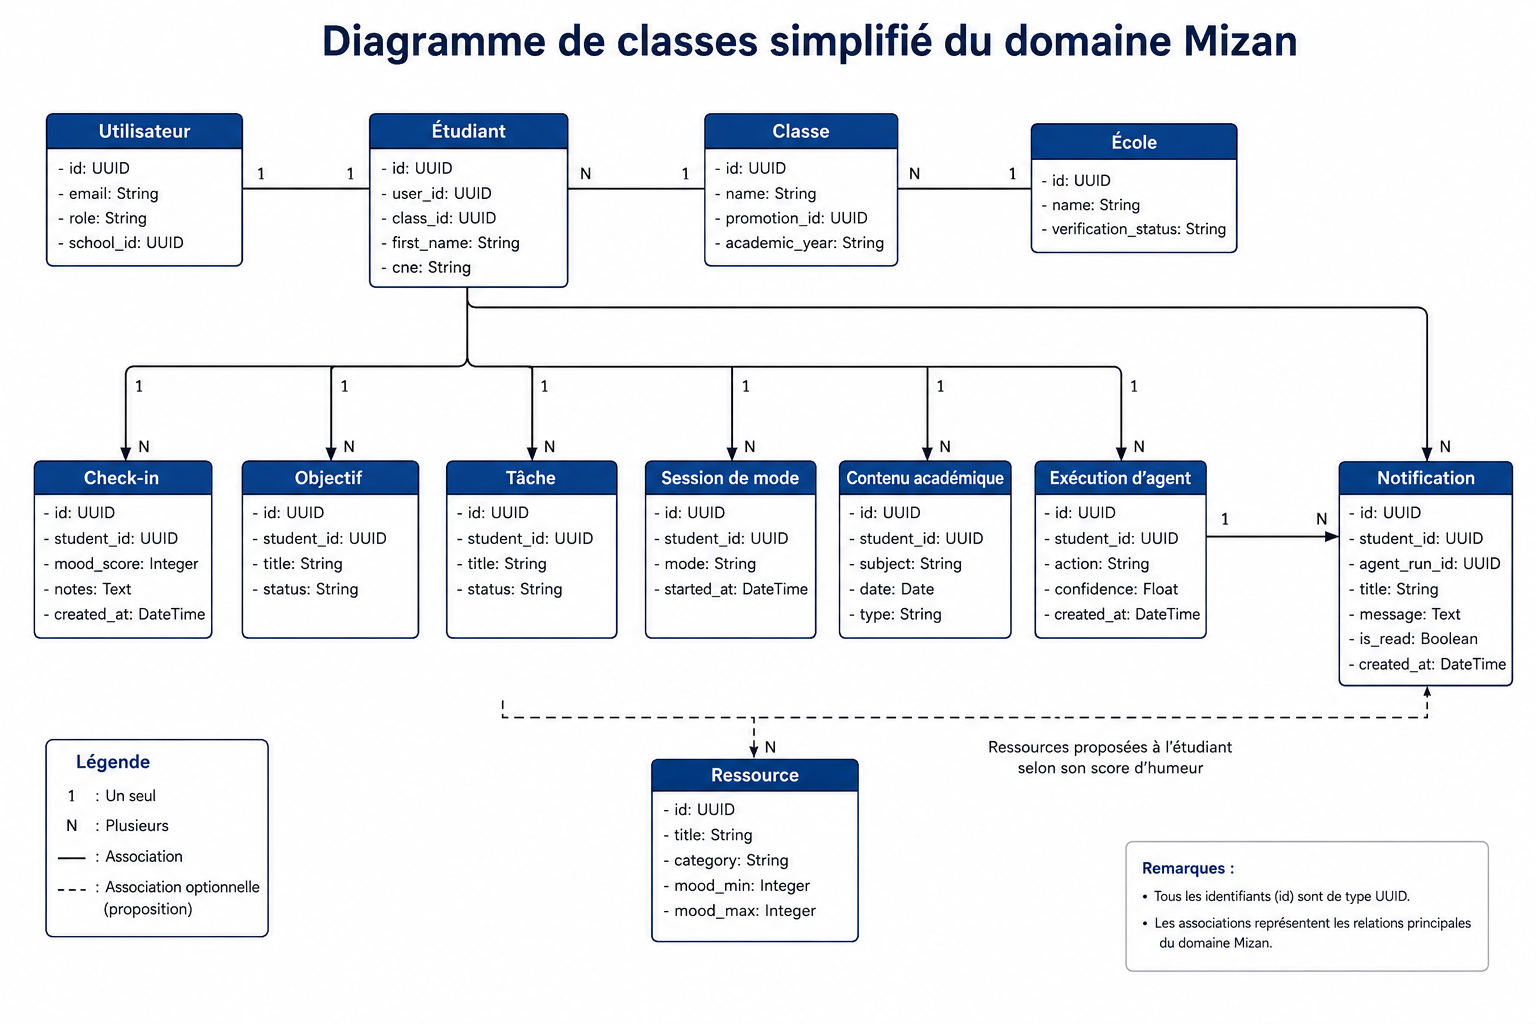
\includegraphics[width=0.92\textheight,height=0.92\textwidth,keepaspectratio]{figures/uml-class.png}}}
}{%
\IfFileExists{figures/diagramme_classes_mizan.png}{%
\makebox[\textwidth][c]{\rotatebox{90}{\includegraphics[width=0.92\textheight,height=0.92\textwidth,keepaspectratio]{figures/diagramme_classes_mizan.png}}}
}{%
\resizebox{0.98\textwidth}{!}{
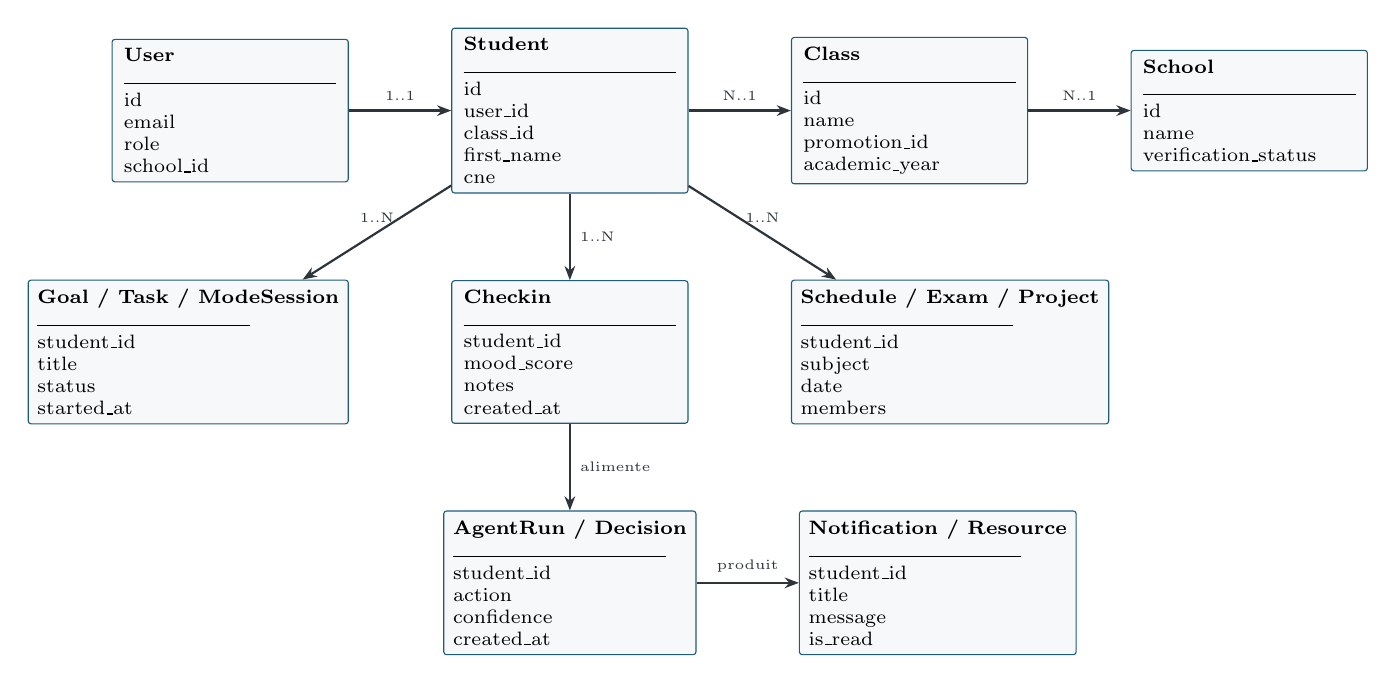
\begin{tikzpicture}[
    umlclass/.style={rectangle, draw=mizanblue, fill=softgray, rounded corners=1pt, minimum width=3.0cm, align=left, font=\scriptsize},
    relation/.style={-{Stealth[length=1.8mm]}, thick, color=darkgray}
]
\node[umlclass] (user) {\textbf{User}\\\rule{2.7cm}{0.25pt}\\id\\email\\role\\school\_id};
\node[umlclass, right=1.3cm of user] (student) {\textbf{Student}\\\rule{2.7cm}{0.25pt}\\id\\user\_id\\class\_id\\first\_name\\cne};
\node[umlclass, right=1.3cm of student] (class) {\textbf{Class}\\\rule{2.7cm}{0.25pt}\\id\\name\\promotion\_id\\academic\_year};
\node[umlclass, right=1.3cm of class] (school) {\textbf{School}\\\rule{2.7cm}{0.25pt}\\id\\name\\verification\_status};
\node[umlclass, below=1.1cm of student] (checkin) {\textbf{Checkin}\\\rule{2.7cm}{0.25pt}\\student\_id\\mood\_score\\notes\\created\_at};
\node[umlclass, right=1.3cm of checkin] (academic) {\textbf{Schedule / Exam / Project}\\\rule{2.7cm}{0.25pt}\\student\_id\\subject\\date\\members};
\node[umlclass, left=1.3cm of checkin] (goal) {\textbf{Goal / Task / ModeSession}\\\rule{2.7cm}{0.25pt}\\student\_id\\title\\status\\started\_at};
\node[umlclass, below=1.1cm of checkin] (agent) {\textbf{AgentRun / Decision}\\\rule{2.7cm}{0.25pt}\\student\_id\\action\\confidence\\created\_at};
\node[umlclass, right=1.3cm of agent] (notification) {\textbf{Notification / Resource}\\\rule{2.7cm}{0.25pt}\\student\_id\\title\\message\\is\_read};
\draw[relation] (user) -- node[above, font=\tiny]{1..1} (student);
\draw[relation] (student) -- node[above, font=\tiny]{N..1} (class);
\draw[relation] (class) -- node[above, font=\tiny]{N..1} (school);
\draw[relation] (student) -- node[right, font=\tiny]{1..N} (checkin);
\draw[relation] (student) -- node[above, font=\tiny]{1..N} (goal);
\draw[relation] (student) -- node[above, font=\tiny]{1..N} (academic);
\draw[relation] (checkin) -- node[right, font=\tiny]{alimente} (agent);
\draw[relation] (agent) -- node[above, font=\tiny]{produit} (notification);
\end{tikzpicture}
}
}
}
}
\caption{Diagramme de classes détaillé du domaine Mizan}
\end{figure}

Ce diagramme distingue deux groupes d'entités. Le premier groupe décrit l'identité et l'organisation académique : \texttt{User}, \texttt{Student}, \texttt{Class} et \texttt{School}. Il permet d'assurer le rattachement correct de chaque étudiant à une classe et de limiter les accès selon le rôle de l'utilisateur. Le deuxième groupe décrit le suivi quotidien : check-ins, objectifs, tâches, sessions de mode, ressources, notifications et exécutions de l'agent.

\begin{longtable}{@{}L{0.25\textwidth}L{0.36\textwidth}L{0.29\textwidth}@{}}
\toprule
\textbf{Zone du modèle} & \textbf{Rôle} & \textbf{Impact fonctionnel} \\
\midrule
\endhead
Identité et rôles & Gérer les comptes, droits et profils. & Connexion, accès étudiant, accès administrateur. \\
Structure académique & Relier écoles, classes et étudiants. & Filtrage des données et gestion administrative. \\
Suivi personnel & Stocker check-ins, objectifs, tâches et modes. & Tableau de bord, historique et recommandations. \\
Accompagnement & Relier agent, ressources et notifications. & Conseils contextualisés et actions proposées. \\
\bottomrule
\caption{Lecture fonctionnelle du diagramme de classes}
\end{longtable}

La relation entre \texttt{Student} et les entités de suivi est centrale : elle garantit que les informations personnelles restent attachées au bon profil. Les cardinalités de type \texttt{1..N} montrent qu'un étudiant peut avoir plusieurs check-ins, objectifs, tâches ou notifications. Ce choix correspond à l'usage réel de Mizan, où les données s'accumulent au fil des jours afin de construire un historique exploitable.

\subsubsection{Diagramme de déploiement}
\begin{figure}[H]
\centering
\IfFileExists{figures/mizan-aws.png}{%
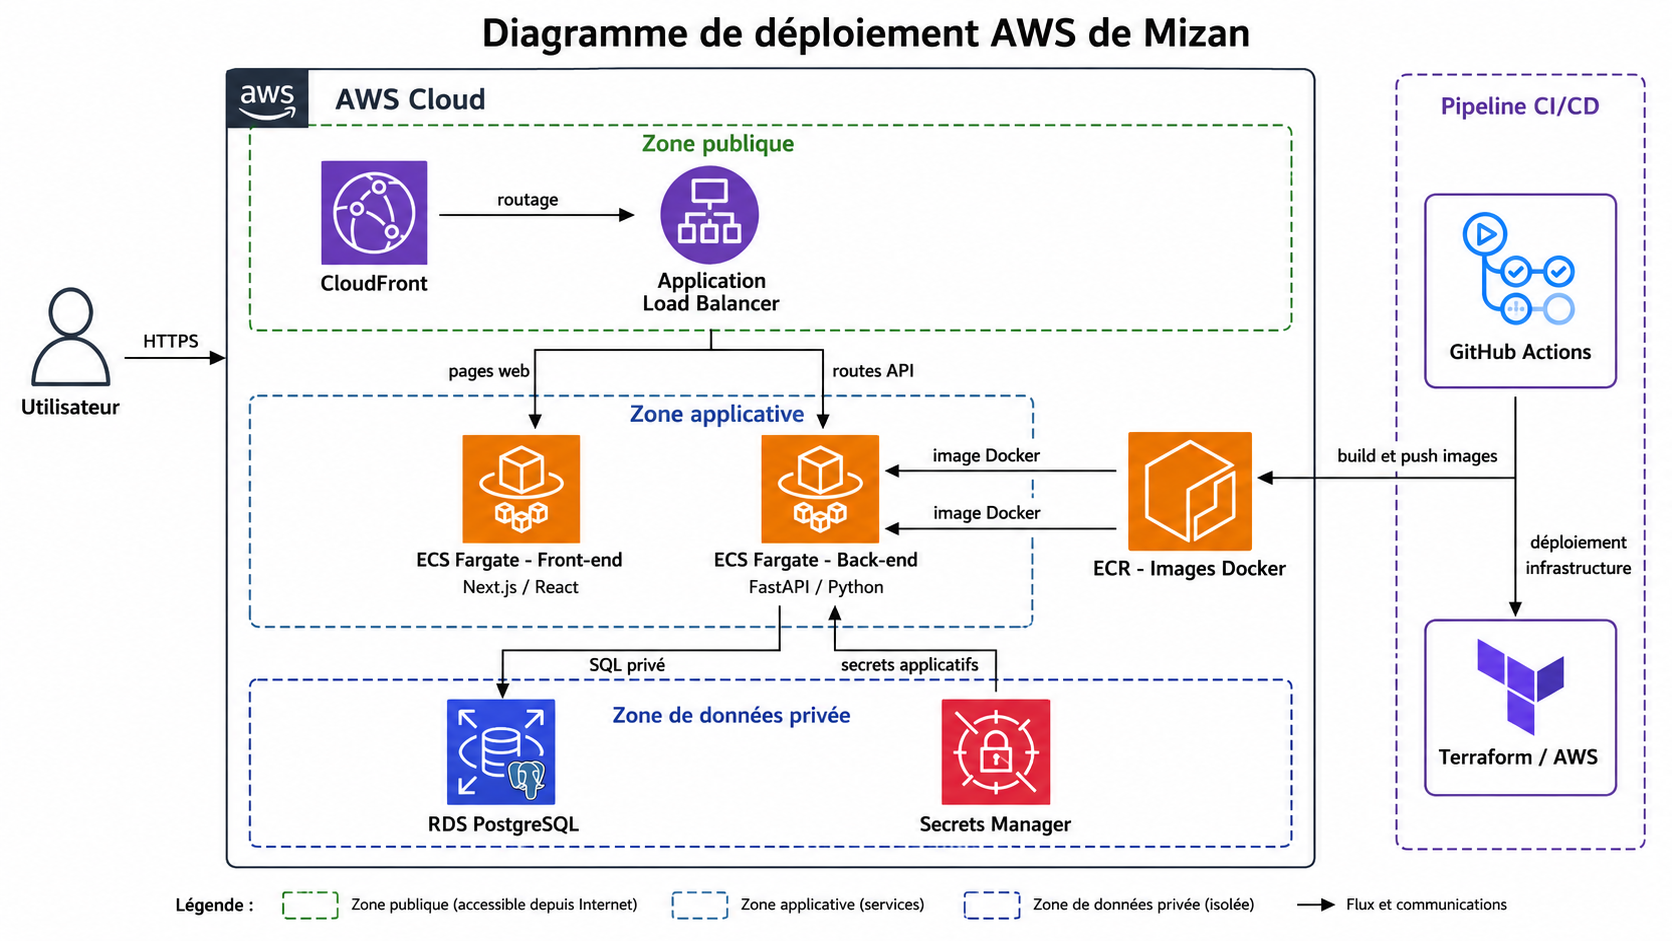
\includegraphics[width=0.96\textwidth]{figures/mizan-aws.png}
}{%
\IfFileExists{figures/diagramme_deploiement_aws_mizan.png}{%
\includegraphics[width=0.96\textwidth]{figures/diagramme_deploiement_aws_mizan.png}
}{%
\resizebox{0.96\textwidth}{!}{
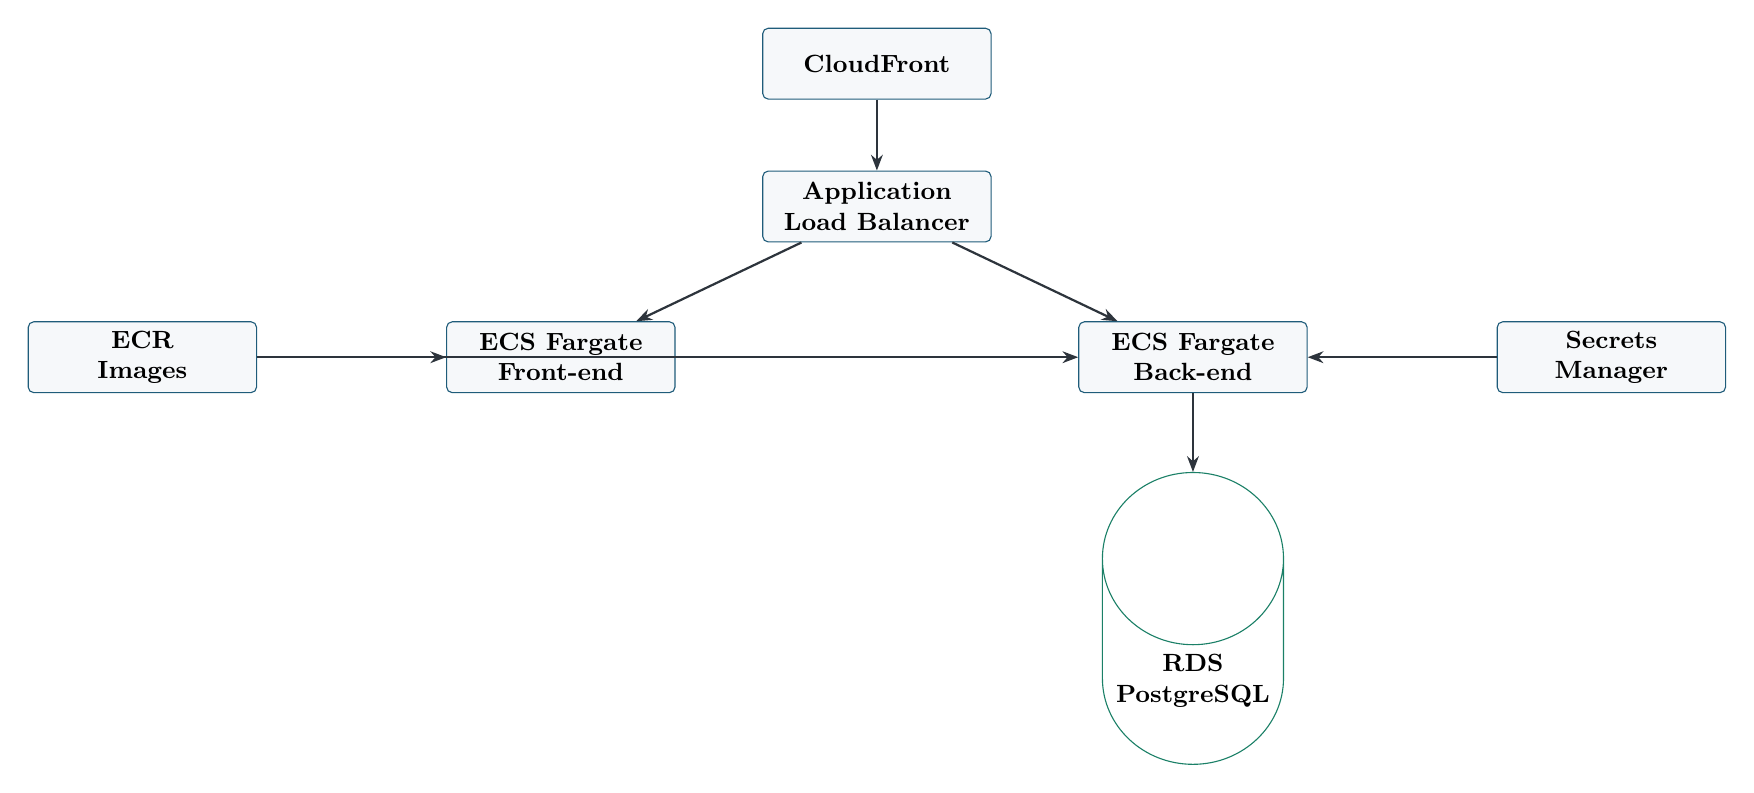
\begin{tikzpicture}[
    nodebox/.style={rectangle, rounded corners=2pt, draw=mizanblue, fill=softgray, minimum width=2.9cm, minimum height=0.9cm, align=center, font=\small\bfseries},
    store/.style={cylinder, shape border rotate=90, draw=mizangreen, fill=white, minimum width=2.3cm, minimum height=1.1cm, align=center, font=\small\bfseries},
    arrow/.style={-{Stealth[length=2mm]}, thick, color=darkgray}
]
\node[nodebox] (cf) {CloudFront};
\node[nodebox, below=0.9cm of cf] (alb) {Application\\Load Balancer};
\node[nodebox, below left=1.0cm and 1.1cm of alb] (front) {ECS Fargate\\Front-end};
\node[nodebox, below right=1.0cm and 1.1cm of alb] (back) {ECS Fargate\\Back-end};
\node[store, below=1.0cm of back] (rds) {RDS\\PostgreSQL};
\node[nodebox, left=2.4cm of front] (ecr) {ECR\\Images};
\node[nodebox, right=2.4cm of back] (secrets) {Secrets\\Manager};
\draw[arrow] (cf) -- (alb);
\draw[arrow] (alb) -- (front);
\draw[arrow] (alb) -- (back);
\draw[arrow] (back) -- (rds);
\draw[arrow] (ecr) -- (front);
\draw[arrow] (ecr) -- (back);
\draw[arrow] (secrets) -- (back);
\end{tikzpicture}
}
}
}
\caption{Diagramme de déploiement AWS}
\end{figure}

Le diagramme de déploiement présente l'architecture cible prévue pour rendre la solution accessible de manière structurée. CloudFront représente le point d'entrée public, tandis que l'Application Load Balancer oriente les requêtes vers le front-end ou vers l'API. Les services front-end et back-end sont isolés afin de pouvoir les faire évoluer séparément. La base PostgreSQL reste dans une zone privée, accessible uniquement par le back-end, ce qui réduit l'exposition des données.

\begin{longtable}{@{}L{0.25\textwidth}L{0.36\textwidth}L{0.29\textwidth}@{}}
\toprule
\textbf{Composant} & \textbf{Responsabilité} & \textbf{Justification} \\
\midrule
\endhead
CloudFront & Point d'accès public et diffusion frontale. & Améliorer l'accès utilisateur et préparer le HTTPS. \\
Load Balancer & Routage vers les services applicatifs. & Séparer les routes web et API. \\
ECS Fargate front-end & Exécution de l'application web. & Déployer l'interface sans gérer de serveur manuel. \\
ECS Fargate back-end & Exécution de l'API FastAPI. & Isoler les règles métier et les accès base. \\
RDS PostgreSQL & Persistance relationnelle. & Centraliser les données critiques dans un stockage managé. \\
Secrets Manager & Gestion des secrets sensibles. & Éviter les clés et mots de passe dans le code. \\
\bottomrule
\caption{Rôle des composants de déploiement}
\end{longtable}

Cette architecture cible reste cohérente avec les exigences non fonctionnelles : sécurité, maintenabilité, évolutivité et séparation des responsabilités. Elle permet aussi de préparer un passage progressif vers une exploitation plus complète, avec supervision, journaux structurés et contrôle des variables d'environnement.

\subsection{Conception des interfaces}
\subsubsection*{Logique générale}
\addcontentsline{toc}{subsubsection}{Logique générale}
La conception des interfaces repose sur une séparation claire entre les usages étudiants et les usages administratifs. L'étudiant doit accéder rapidement aux informations qui l'aident dans sa journée : humeur, sommeil, priorités, objectifs, tâches, modes de travail, notifications et recommandations. L'administrateur, au contraire, a besoin d'écrans plus structurés pour gérer des listes, importer des données, consulter des classes et maintenir les contenus académiques.

Cette différence influence directement l'organisation visuelle. Les écrans étudiants privilégient les cartes de synthèse, les actions rapides et les formulaires courts. Les écrans administrateur privilégient les tableaux, les filtres, les boutons d'action et les formulaires de gestion. Le but n'est pas de multiplier les pages, mais de réduire l'effort mental pour chaque type d'utilisateur.

\subsubsection*{Parcours utilisateur}
\addcontentsline{toc}{subsubsection}{Parcours utilisateur}
Le parcours étudiant commence par la connexion, puis le tableau de bord. L'étudiant peut réaliser un check-in, consulter ses tâches, suivre ses objectifs et demander de l'aide à l'assistant. Le parcours administrateur commence par la connexion à l'espace admin, puis la gestion des structures, étudiants et contenus.

\begin{longtable}{@{}L{0.24\textwidth}L{0.32\textwidth}L{0.34\textwidth}@{}}
\toprule
\textbf{Profil} & \textbf{Besoin principal} & \textbf{Réponse d'interface} \\
\midrule
\endhead
Étudiant & Comprendre sa journée rapidement. & Dashboard synthétique, check-in court, objectifs visibles. \\
Étudiant en période chargée & Prioriser sans perdre du temps. & Rappels, échéances proches, assistant et plan d'action. \\
Administrateur d'école & Gérer classes et étudiants. & Tableaux, import CSV, actions de création et modification. \\
Administrateur global & Suivre les établissements. & Écrans de supervision et validation. \\
\bottomrule
\caption{Correspondance entre profils et interfaces}
\end{longtable}

\subsubsection*{Ergonomie et navigation}
\addcontentsline{toc}{subsubsection}{Ergonomie et navigation}
L'ergonomie repose sur des pages dédiées, une navigation claire, des formulaires courts et des tableaux synthétiques. L'application mobile facilite les usages rapides, notamment les check-ins.

Les interfaces sont pensées selon la fréquence d'utilisation. Les actions quotidiennes, comme le check-in ou la consultation du tableau de bord, doivent être accessibles rapidement. Les actions administratives, plus structurées, privilégient les tableaux, formulaires et imports. Cette différence permet de proposer une expérience simple à l'étudiant tout en gardant une gestion complète pour l'administrateur.

\begin{longtable}{@{}L{0.25\textwidth}L{0.37\textwidth}L{0.28\textwidth}@{}}
\toprule
\textbf{Parcours} & \textbf{Écrans concernés} & \textbf{Point d'attention ergonomique} \\
\midrule
\endhead
Connexion et activation & Login, activation, mot de passe. & Messages clairs et étapes courtes. \\
Check-in quotidien & Check-in matin, check-in soir, historique. & Formulaire rapide et feedback immédiat. \\
Suivi personnel & Dashboard, objectifs, tâches, modes. & Synthèse visuelle et priorité aux informations utiles. \\
Accompagnement IA & Chat, scénarios, contrats d'action. & Réponses lisibles et actions concrètes. \\
Administration & Classes, étudiants, contenus, ressources. & Tableaux structurés, filtres et imports. \\
\bottomrule
\caption{Parcours utilisateur et exigences d'interface}
\end{longtable}

\subsubsection*{Organisation des écrans}
\addcontentsline{toc}{subsubsection}{Organisation des écrans}
L'organisation des écrans suit une logique de priorité. Les informations les plus fréquentes apparaissent en premier : état du jour, objectifs, tâches, échéances proches et notifications. Les informations plus détaillées, comme l'historique ou les ressources, restent accessibles par navigation. Cette hiérarchie évite de transformer le tableau de bord en page trop dense.

\begin{longtable}{@{}L{0.24\textwidth}L{0.34\textwidth}L{0.32\textwidth}@{}}
\toprule
\textbf{Écran} & \textbf{Contenu principal} & \textbf{Justification} \\
\midrule
\endhead
Dashboard étudiant & Humeur, sommeil, tâches, objectifs, échéances. & Donner une vision immédiate de la journée. \\
Check-in & Questions courtes matin/soir. & Favoriser une saisie régulière. \\
Objectifs et tâches & Progression, statut, actions rapides. & Aider l'étudiant à suivre ses engagements. \\
Assistant & Conversation, recommandations, plans d'action. & Transformer les données en conseils exploitables. \\
Administration & Classes, étudiants, contenus, ressources. & Centraliser la gestion pédagogique. \\
\bottomrule
\caption{Organisation logique des écrans}
\end{longtable}

\subsubsection*{Cohérence avec les cas d'utilisation}
\addcontentsline{toc}{subsubsection}{Cohérence avec les cas d'utilisation}
Chaque interface correspond à un cas d'utilisation identifié : check-in, suivi des objectifs, gestion institutionnelle, import, consultation des statistiques et dialogue avec l'assistant.

La cohérence est assurée par la correspondance entre acteurs, besoins et écrans. Le check-in répond au besoin de suivi quotidien. Le dashboard répond au besoin de synthèse. Les pages d'objectifs et de tâches répondent au besoin d'organisation. L'espace administrateur répond au besoin de gestion académique. Enfin, l'assistant répond au besoin d'accompagnement personnalisé. Cette logique évite d'ajouter des interfaces sans lien direct avec les besoins exprimés.

% ===========================================================
% CHAPITRE 4
% ===========================================================

\section{Réalisation et Implémentation}
\subsection{Environnement de développement}
\begin{table}[H]
\centering
\begin{tabularx}{\textwidth}{@{}L{0.28\textwidth}Y@{}}
\toprule
\textbf{Élément} & \textbf{Valeur} \\
\midrule
Système d'exploitation & Linux pour le développement local. \\
IDE / éditeur & Éditeur de code moderne avec terminal intégré. \\
Versions principales & Python 3.12, Node.js 20, Next.js, React, Expo, PostgreSQL. \\
Configuration matérielle & Poste de développement standard et architecture cloud cible. \\
\bottomrule
\end{tabularx}
\caption{Environnement de développement}
\end{table}

\subsection{Architecture réalisée}
L'architecture réalisée respecte la séparation des composants présentée dans les diagrammes de conception : front-end web, application mobile, API FastAPI, base PostgreSQL et intégrations externes. La structure réelle du code sépare clairement les applications et facilite les tests indépendants.

Le back-end regroupe les routes HTTP, la configuration, la sécurité, les modèles SQLAlchemy, les schémas Pydantic et les services métier. Le front-end web regroupe les pages étudiant, les pages administrateur, les composants UI et la couche API. L'application mobile reprend les usages rapides, notamment l'accès au back-end depuis un téléphone ou un émulateur. Cette séparation permet de faire évoluer un composant sans bloquer les autres.

\begin{longtable}{@{}L{0.24\textwidth}L{0.34\textwidth}L{0.32\textwidth}@{}}
\toprule
\textbf{Composant} & \textbf{Responsabilité réalisée} & \textbf{Exemple de livrable} \\
\midrule
\endhead
Back-end & API, règles métier, sécurité, persistance. & Routes \texttt{/api/v1}, services et modèles. \\
Front-end web & Interface étudiant et administration. & Pages dashboard, check-in, classes et ressources. \\
Mobile & Accès rapide au suivi étudiant. & Application Expo React Native. \\
Base de données & Stockage relationnel des entités. & Tables étudiants, check-ins, objectifs, notifications. \\
Infrastructure & Préparation du déploiement et automatisation. & Docker, Terraform et GitHub Actions. \\
\bottomrule
\caption{Correspondance entre conception et réalisation}
\end{longtable}

\subsection{Implémentation des fonctionnalités}
\subsubsection*{Authentification et contrôle d'accès}
\addcontentsline{toc}{subsubsection}{Authentification et contrôle d'accès}
L'authentification utilise des jetons JWT, des jetons de rafraîchissement et des dépendances FastAPI pour identifier l'utilisateur courant. Les rôles \texttt{ADMIN} et \texttt{STUDENT} protègent les routes sensibles.

Lorsqu'un utilisateur se connecte, l'API vérifie ses identifiants, génère un jeton d'accès et un jeton de rafraîchissement. Le front-end ajoute ensuite automatiquement le jeton d'accès aux requêtes. Si le jeton expire, la couche API tente un renouvellement avant de rediriger l'utilisateur vers la page de connexion.

\subsubsection*{Gestion des utilisateurs}
\addcontentsline{toc}{subsubsection}{Gestion des utilisateurs}
La gestion des utilisateurs couvre l'activation, la connexion, la création des étudiants, l'import CSV et le rattachement aux classes.

L'import CSV répond à un besoin pratique : créer plusieurs étudiants sans saisie manuelle répétitive. Les données importées doivent être validées avant insertion afin d'éviter les comptes incomplets ou les rattachements à des classes inexistantes.

\subsubsection*{Gestion des données métier}
\addcontentsline{toc}{subsubsection}{Gestion des données métier}
Les données métier incluent écoles, filières, promotions, classes, étudiants, emplois du temps, examens, projets, check-ins, objectifs, tâches, modes, ressources et notifications.

Ces données sont organisées autour du profil étudiant. Les emplois du temps, examens et projets enrichissent le contexte académique. Les check-ins, objectifs, tâches et modes décrivent l'état personnel et l'organisation quotidienne. Les ressources et notifications servent à transformer ce contexte en accompagnement concret.

\subsubsection*{Opérations CRUD}
\addcontentsline{toc}{subsubsection}{Opérations CRUD}
Les opérations CRUD sont exposées par des routes REST. Les schémas Pydantic valident les entrées et les services appliquent les règles métier avant la persistance.

Cette approche limite les responsabilités de chaque couche. Les routes reçoivent la requête, les schémas contrôlent la forme des données, les services appliquent les règles et les modèles assurent la persistance. Elle rend le code plus testable et plus lisible.

\subsubsection*{Export et notifications}
\addcontentsline{toc}{subsubsection}{Export et notifications}
Le système de notifications permet la consultation REST et la livraison temps réel pour les rappels et actions autonomes.

Les notifications sont utiles pour signaler un rappel de check-in, une recommandation de pause, une échéance ou une action proposée par l'assistant. Elles doivent rester pertinentes afin de ne pas créer de surcharge supplémentaire pour l'étudiant.

\subsection{Intégration avec la base de données}
\subsubsection*{Connexion et ORM}
\addcontentsline{toc}{subsubsection}{Connexion et ORM}
La connexion à PostgreSQL est gérée par SQLAlchemy en mode asynchrone. Alembic versionne les migrations afin de garder une évolution contrôlée du schéma.

\subsubsection*{Requêtes principales}
\addcontentsline{toc}{subsubsection}{Requêtes principales}
Les requêtes principales concernent la récupération du contexte étudiant, l'historique des check-ins, les objectifs actifs, les échéances académiques et les indicateurs de tableau de bord.

\begin{longtable}{@{}L{0.30\textwidth}L{0.30\textwidth}L{0.30\textwidth}@{}}
\toprule
\textbf{Donnée consultée} & \textbf{Utilisation} & \textbf{Module consommateur} \\
\midrule
\endhead
Historique des check-ins & Suivre l'évolution de l'humeur et du sommeil. & Dashboard, analytics, assistant. \\
Examens et projets & Identifier les échéances proches. & Assistant, notifications, dashboard. \\
Objectifs et tâches & Mesurer la progression quotidienne. & Dashboard, agent, pages objectifs. \\
Modes de travail & Comprendre la répartition du temps. & Historique, statistiques. \\
Ressources & Proposer un soutien adapté. & Assistant, notifications. \\
\bottomrule
\caption{Utilisation des données principales}
\end{longtable}

\subsubsection*{Sécurité des accès}
\addcontentsline{toc}{subsubsection}{Sécurité des accès}
Les accès sont sécurisés par rôles, par validation de l'utilisateur courant et par scoping des administrateurs selon l'établissement.

Cette logique réduit les risques d'accès croisé entre établissements. Un administrateur ne doit pas manipuler les données d'une école qui ne lui appartient pas. De même, un étudiant ne doit consulter que ses propres informations.

\subsection{Sécurité et contrôle d'accès}
La sécurité du projet repose sur plusieurs niveaux :
\begin{itemize}
    \item authentification par jetons JWT ;
    \item mots de passe hachés côté serveur ;
    \item contrôle du rôle \texttt{ADMIN} ou \texttt{STUDENT} selon les routes ;
    \item validation stricte des données avec Pydantic ;
    \item limites de taille pour les fichiers image, audio et CSV ;
    \item rejet des secrets faibles en production ;
    \item CORS restreint en environnement de production.
\end{itemize}

\subsection{Plan de validation et qualité}
Le plan de validation du projet repose sur une combinaison de vérifications automatiques et de scénarios fonctionnels. Les tests automatiques permettent de détecter rapidement les régressions dans le back-end, tandis que les commandes de lint et de build vérifient la cohérence des applications front-end et mobile. Cette démarche est importante car Mizan comporte plusieurs interfaces qui consomment la même API.

\begin{longtable}{@{}L{0.24\textwidth}L{0.34\textwidth}L{0.32\textwidth}@{}}
\toprule
\textbf{Zone validée} & \textbf{Vérification} & \textbf{Objectif} \\
\midrule
\endhead
Back-end & Compilation Python et tests Pytest. & Vérifier les services, contrats et règles métier. \\
Front-end web & Lint et build Next.js. & Détecter les erreurs TypeScript, React et routage. \\
Mobile & Typecheck TypeScript. & Vérifier la cohérence des types et appels API. \\
Déploiement & Tests de readiness et configuration production. & Refuser les secrets faibles et paramètres incomplets. \\
Sécurité fichiers & Validation des extensions, types MIME et tailles. & Éviter les fichiers dangereux ou trop volumineux. \\
Assistant & Tests du fallback et de l'orchestration. & Maintenir une réponse utile même sans fournisseur externe. \\
\bottomrule
\caption{Stratégie de tests et validation}
\end{longtable}

\begin{lstlisting}[language=bash]
# Validation back-end
cd mizan-backend
python -m compileall -q app main.py tests
python -m pytest

# Validation front-end web
cd ../mizan-frontend
npm run lint
npm run build

# Validation mobile
cd ../mizan-mobile-app
npm run typecheck
\end{lstlisting}

Les scénarios fonctionnels à vérifier couvrent le parcours minimal : activation ou connexion d'un étudiant, réalisation d'un check-in, consultation du tableau de bord, création d'un objectif, échange avec l'assistant, puis consultation d'une notification. Côté administration, la validation concerne la création d'une structure institutionnelle, l'ajout ou l'import d'étudiants, l'ajout d'un examen et la consultation d'indicateurs.

\begin{longtable}{@{}L{0.28\textwidth}L{0.34\textwidth}L{0.28\textwidth}@{}}
\toprule
\textbf{Scénario validé} & \textbf{Critère de réussite} & \textbf{Risque couvert} \\
\midrule
\endhead
Connexion étudiant & Jeton reçu et redirection vers le dashboard. & Blocage d'accès ou erreur d'authentification. \\
Check-in matin & Données sauvegardées et historique mis à jour. & Perte de données quotidiennes. \\
Assistant & Réponse générée ou fallback local affiché. & Dépendance totale à un service externe. \\
Import étudiants & Lignes valides créées et erreurs signalées. & Données administratives incohérentes. \\
Contrôle des rôles & Route admin inaccessible à un étudiant. & Accès non autorisé. \\
\bottomrule
\caption{Matrice de validation fonctionnelle}
\end{longtable}

\subsection{Préparation du déploiement et exploitation}
La préparation du déploiement est organisée autour de Docker, Terraform et GitHub Actions. Docker fournit un environnement reproductible pour le front-end et le back-end. Terraform décrit l'infrastructure AWS cible, notamment le réseau, les services ECS, le registre ECR, la base RDS, CloudFront et l'Application Load Balancer. GitHub Actions prépare les étapes de vérification, construction et déploiement.

\begin{longtable}{@{}L{0.27\textwidth}L{0.33\textwidth}L{0.30\textwidth}@{}}
\toprule
\textbf{Élément d'exploitation} & \textbf{Rôle} & \textbf{Exemple de configuration} \\
\midrule
\endhead
Variables d'environnement & Adapter l'application à chaque environnement. & \texttt{DATABASE\_URL}, \texttt{JWT\_SECRET}, \texttt{CORS\_ORIGINS}. \\
Secrets applicatifs & Protéger clés et mots de passe. & Secrets AWS ou variables GitHub Actions. \\
Images Docker & Emballer les applications. & Images back-end et front-end prévues pour ECR. \\
Migrations Alembic & Faire évoluer le schéma SQL. & Exécution contrôlée avant mise en production. \\
Endpoint de santé & Vérifier la disponibilité du service. & Route de health check prévue pour l'infrastructure. \\
\bottomrule
\caption{Éléments de déploiement et exploitation}
\end{longtable}

En exploitation, les points de vigilance principaux sont la surveillance des erreurs API, la disponibilité de la base de données, la validité des secrets, la taille des fichiers envoyés et la stabilité des appels vers les fournisseurs externes. Une amélioration future consiste à ajouter une observabilité plus complète : journaux structurés, métriques applicatives, alertes et suivi des temps de réponse par route.

\subsection{Difficultés rencontrées}
\subsubsection*{Problèmes techniques et d'intégration}
\addcontentsline{toc}{subsubsection}{Problèmes techniques et d'intégration}
Les principales difficultés concernent l'intégration de l'IA avec un mode de secours, la cohérence entre le web et le mobile, la gestion des secrets, la validation des fichiers et la préparation du déploiement cloud.

Une autre difficulté a été la construction d'un contexte suffisamment riche pour l'assistant sans rendre le système trop complexe. L'assistant doit recevoir les informations utiles, mais il ne doit pas dépendre d'un nombre excessif de données obligatoires. Il fallait donc prévoir un fonctionnement progressif : plus le contexte est riche, plus la réponse peut être personnalisée, mais l'application doit rester utilisable avec un contexte minimal.

\subsubsection*{Solutions adoptées}
\addcontentsline{toc}{subsubsection}{Solutions adoptées}
Les solutions adoptées sont la modularisation des services, la validation stricte des paramètres, l'utilisation d'un fallback local pour l'IA, la centralisation de la couche API front-end, l'organisation des tests et l'infrastructure décrite par Terraform.

La solution adoptée consiste aussi à séparer les responsabilités. Le service de contexte prépare les données utiles, le service agent produit la réponse, le service notification se charge de la diffusion et les routes gardent un rôle d'orchestration HTTP. Cette organisation limite le couplage et facilite les évolutions futures.

% ===========================================================
% CONCLUSION
% ===========================================================

\section*{Conclusion Générale}
\addcontentsline{toc}{section}{Conclusion Générale}
\subsection*{Bilan du projet}
\addcontentsline{toc}{subsection}{Bilan du projet}
Mizan constitue une solution complète pour accompagner les étudiants dans leur organisation et leur bien-être quotidien. Le projet associe des fonctionnalités académiques, personnelles et intelligentes dans une architecture moderne : FastAPI, Next.js, Expo React Native, PostgreSQL, Docker, Terraform et architecture AWS cible.

Le travail réalisé a permis de passer d'un besoin général, celui d'aider l'étudiant à mieux gérer son quotidien, à une solution structurée composée de modules cohérents. L'application ne se limite pas à une simple liste de tâches : elle relie le contexte académique, les check-ins, les objectifs, les notifications et l'assistant intelligent. Cette combinaison donne au projet une valeur particulière, car elle aborde à la fois l'organisation, le suivi personnel et l'accompagnement.

\subsection*{Réponse à la problématique}
\addcontentsline{toc}{subsection}{Réponse à la problématique}
La solution répond à la problématique en centralisant les informations académiques et les signaux de bien-être dans une même plateforme. Elle permet de produire des tableaux de bord, des recommandations et des notifications contextualisées.

La réponse proposée repose sur trois axes. Le premier est la centralisation : l'étudiant retrouve ses informations importantes dans un espace unique. Le deuxième est la contextualisation : les recommandations prennent en compte les objectifs, les échéances, les check-ins et les données disponibles. Le troisième est la séparation des rôles : l'étudiant agit sur son suivi personnel, tandis que l'administrateur gère les données académiques nécessaires au bon fonctionnement de la plateforme.

\subsection*{Objectifs atteints}
\addcontentsline{toc}{subsection}{Objectifs atteints}
Les objectifs atteints concernent l'authentification, la gestion institutionnelle, les profils étudiants, les check-ins, les objectifs, les modes, l'assistant, les ressources et les notifications.

Au-delà de la réalisation fonctionnelle, le projet a permis de mettre en place une logique de traçabilité entre besoins, conception et implémentation. Chaque module principal répond à un besoin identifié : les check-ins pour le suivi quotidien, les objectifs et tâches pour l'organisation, les contenus académiques pour le contexte, l'assistant pour l'accompagnement et les tableaux de bord pour la synthèse.

\subsection*{Limites du travail réalisé}
\addcontentsline{toc}{subsection}{Limites du travail réalisé}
Certaines fonctionnalités IA dépendent de clés externes et de la disponibilité du fournisseur. L'application mobile peut encore être enrichie pour couvrir toutes les fonctions du web. Les tests end-to-end utilisateur peuvent également être renforcés.

Une autre limite concerne l'évaluation réelle de l'impact sur les étudiants. La plateforme fournit des outils de suivi et d'accompagnement, mais son efficacité doit être mesurée sur une période d'utilisation plus longue, avec des retours utilisateurs et des indicateurs qualitatifs. La qualité des recommandations dépend également de la régularité des check-ins et de la richesse des données académiques renseignées.

Il faut également souligner que les données de bien-être exigent une attention particulière. Même si la solution prévoit des mécanismes de sécurité, une version plus avancée devrait formaliser davantage le consentement, la durée de conservation des données, l'export et la suppression des informations personnelles. Ces éléments sont importants pour renforcer la confiance des utilisateurs.

\subsection*{Perspectives d'amélioration}
\addcontentsline{toc}{subsection}{Perspectives d'amélioration}
Les perspectives prioritaires sont l'ajout de tests end-to-end, l'amélioration des tableaux de bord, la parité fonctionnelle mobile, les notifications natives et une politique explicite de consentement et d'export des données.

À moyen terme, Mizan pourrait intégrer une analyse plus avancée des tendances, un calendrier partagé, des exports PDF, des recommandations personnalisées par période académique et une meilleure prise en charge du travail en groupe. Sur le plan technique, l'ajout d'une observabilité complète et d'un pipeline de déploiement multi-environnements renforcerait la fiabilité de la solution.

\begin{longtable}{@{}L{0.28\textwidth}L{0.36\textwidth}L{0.26\textwidth}@{}}
\toprule
\textbf{Perspective} & \textbf{Description} & \textbf{Apport attendu} \\
\midrule
\endhead
Tests end-to-end & Automatiser les parcours étudiant et administrateur. & Réduire les régressions fonctionnelles. \\
Mobile complet & Couvrir davantage de fonctionnalités web côté mobile. & Améliorer l'usage quotidien. \\
Consentement et données & Ajouter des règles explicites d'export, suppression et conservation. & Renforcer la confiance et la conformité. \\
Analytique avancée & Étudier les tendances par période, classe ou type d'échéance. & Aider à repérer les périodes de surcharge. \\
Notifications natives & Ajouter des rappels mobiles mieux intégrés. & Améliorer la régularité des check-ins. \\
Observabilité & Ajouter journaux structurés, métriques et alertes. & Faciliter le suivi technique. \\
\bottomrule
\caption{Perspectives d'amélioration de Mizan}
\end{longtable}

Ces perspectives ne changent pas l'objectif initial du projet ; elles l'approfondissent. La priorité reste de conserver une solution utile et simple pour l'étudiant. Les améliorations futures doivent donc être évaluées selon leur capacité à réduire la charge mentale, clarifier les priorités et rendre les informations plus exploitables.

\subsection*{Apport personnel et professionnel}
\addcontentsline{toc}{subsection}{Apport personnel et professionnel}
Ce projet a permis de consolider des compétences en analyse des besoins, conception UML, architecture C4, développement back-end, développement front-end, développement mobile, sécurité applicative, organisation des tests et préparation du déploiement cloud.

Sur le plan personnel, Mizan a permis de travailler sur un sujet qui combine technique et utilité concrète. La réalisation a demandé une vision globale : comprendre le besoin, structurer les données, concevoir les interfaces, organiser les modules et préparer une architecture évolutive. Sur le plan professionnel, ce projet a renforcé la pratique du développement full-stack, de la documentation technique et de la modélisation logicielle.

% ===========================================================
% ANNEXES
% ===========================================================

\newpage
\section*{Annexe A -- Glossaire Technique}
\addcontentsline{toc}{section}{Annexe A -- Glossaire Technique}
\begin{longtable}{@{}L{0.25\textwidth}L{0.65\textwidth}@{}}
\toprule
\textbf{Terme} & \textbf{Définition} \\
\midrule
\endhead
Back-end & Partie serveur responsable de l'API, des règles métier et de la base de données. \\
Front-end & Interface utilisée par l'utilisateur depuis le navigateur. \\
Check-in & Saisie régulière permettant de suivre l'humeur, le sommeil et le bilan de l'étudiant. \\
Conteneur & Unité d'exécution Docker embarquant une application et ses dépendances. \\
Migration & Script de versionnement permettant de faire évoluer le schéma de base de données. \\
\bottomrule
\caption{Glossaire technique}
\end{longtable}

% ===========================================================
% BIBLIOGRAPHIE / WEBOGRAPHIE
% ===========================================================

\section*{Bibliographie / Webographie}
\addcontentsline{toc}{section}{Bibliographie / Webographie}
\begin{itemize}
    \item Documentation FastAPI : \url{https://fastapi.tiangolo.com/}
    \item Documentation Next.js : \url{https://nextjs.org/docs}
    \item Documentation Expo : \url{https://docs.expo.dev/}
    \item Documentation SQLAlchemy : \url{https://docs.sqlalchemy.org/}
    \item \href{https://registry.terraform.io/providers/hashicorp/aws/latest/docs}{Documentation Terraform AWS Provider}.
    \item Documentation locale du projet Mizan : \texttt{README.md}, \texttt{mizan-backend/README.md}, \texttt{mizan-mobile-app/README.md}, \texttt{DEPLOYMENT\_README.md}.
\end{itemize}

\end{document}
